\documentclass[8pt]{beamer}

\newif\ifplacelogo % create a new conditional
\placelogotrue % set it to true

\usetheme{Warsaw}
\usecolortheme{rose}
\usepackage{multicol}
\usepackage{epstopdf}
\usepackage[italic]{hepnames}
\usepackage{tikz}
\usepackage{listings}
\usepackage{times}
\usepackage{amsmath}
\usepackage{verbatim}
\usepackage{hyperref}
\usepackage{bbding}
\usepackage{upgreek}
\lstset{breakatwhitespace,
language=C++,
columns=fullflexible,
keepspaces,
breaklines,
tabsize=3, 
showstringspaces=false,
extendedchars=true}

% TikZ includes!!!
\usepackage{tikz}
\usetikzlibrary{backgrounds}
\usetikzlibrary{calc}
\tikzstyle{every picture}+=[remember picture]
\input{/home/oviazlo/Desktop/beamerPresentations/myReports/latexHelpScripts/tikzGrid.tex}


\begin{document}

% custom colors
\definecolor{olive}{rgb}{0.3, 0.4, .1}
\definecolor{fore}{RGB}{249,242,215}
\definecolor{back}{RGB}{51,51,51}
\definecolor{title}{RGB}{255,0,90}
\definecolor{dgreen}{rgb}{0.,0.6,0.}
\definecolor{gold}{rgb}{1.,0.84,0.}
\definecolor{JungleGreen}{cmyk}{0.99,0,0.52,0}
\definecolor{BlueGreen}{cmyk}{0.85,0,0.33,0}
\definecolor{RawSienna}{cmyk}{0,0.72,1,0.45}
\definecolor{Magenta}{cmyk}{0,1,0,0}

\definecolor{PixelColor}{RGB}{207,232,139}
\definecolor{SCTColor}{RGB}{167,166,255}
\definecolor{TRTColor}{RGB}{250,224,140}
\definecolor{grayColor}{RGB}{153,153,153}

\newcommand{\yRefPosOne}{0.0}
\newcommand{\xRefPosOne}{0.0}
\newcommand{\yRefPosTwo}{0.0}
\newcommand{\xRefPosTwo}{0.0}
\newcommand{\yRefIncrementOne}{0.0}
\newcommand{\xRefIncrementOne}{0.0}
\newcommand{\yRefIncrementTwo}{0.0}
\newcommand{\xRefIncrementTwo}{0.0}

\graphicspath{ {/home/oviazlo/Desktop/beamerPresentations/FCCee/pictures/plots_FCCweek_workshop/} }


\DeclareGraphicsExtensions{.eps, .pdf, .png}

\newcommand{\myBox}[2][pink] {
    \noindent\colorbox{#1}{
	\textbf{#2}
    }\par
}

% For nice block (provided by Oleh)
\tikzstyle{myBox} = [draw=red, fill=blue!1, very thick,
    rectangle, rounded corners, inner sep=5pt, inner ysep=9pt]
    
\tikzstyle{PixelBox} = [draw=PixelColor, fill=blue!1, very thick,
    rectangle, rounded corners, inner sep=5pt, inner ysep=9pt]
\tikzstyle{SCTBox} = [draw=SCTColor, fill=blue!1, very thick,
    rectangle, rounded corners, inner sep=5pt, inner ysep=9pt]
\tikzstyle{TRTBox} = [draw=TRTColor, fill=blue!1, very thick,
    rectangle, rounded corners, inner sep=5pt, inner ysep=9pt]

% poster advertisement
\newcommand{\myCenterBox}[2][pink] {
   {\centering
    \noindent\colorbox{#1}{
	\textbf{#2}
    }\par
  }
}

\newcommand{\mySmallCenterBox}[2][pink] {
   {\centering
    \noindent\colorbox{#1}{
	\textbf{{\small #2}}
    }\par
  }
}

\newcommand{\myVerySmallCenterBox}[2][pink] {
   {\centering
    \noindent\colorbox{#1}{
	\textbf{{\scriptsize #2}}
    }\par
  }
}

\newcommand{\backupbegin}{
   \newcounter{finalframe}
   \setcounter{finalframe}{\value{framenumber}}
}
\newcommand{\backupend}{
   \setcounter{framenumber}{\value{finalframe}}
}

\newcommand{\myNode}{\tikz[baseline,inner sep=1pt] \node[anchor=base]}

\tikzstyle{fancytitle} =[fill=white!15, text=black]

\definecolor{light-gray}{gray}{0.95}
% poster advertisement


\title[ CLD detector model overview  \hspace{16.5em}\insertframenumber/
\inserttotalframenumber]{ CLD detector model overview of layout and performances}


	\author[Oleksandr Viazlo]{Oleksandr Viazlo \\ 
% 	{\small ???}
	}
	\institute{\small CERN\\} 
	
       
	\date{10 April 2018}

% 	\logo{ \ifplacelogo \includegraphics[height=1.8cm]{./ID_week2/lund_uni-logo_s.pdf} \hspace{0.4cm} \fi}

	
   	\frame{\titlepage}

   	

\placelogofalse

% %*****************************************************************************
% \begin{frame}
% \frametitle{Introduction} 
% 
% \renewcommand{\yRefPosOne}{0}
% \renewcommand{\xRefPosOne}{5.3}
% \renewcommand{\xRefIncrementOne}{5.5}
% 
% \begin{tikzpicture}[overlay]
% 
% 
% %% HELPER draw advanced helping grid with axises:
% % \draw(-0.5,-4) to[grid with coordinates] (11.5,4);
% 
% \end{tikzpicture}
% \end{frame}
% %*****************************************************************************
% %*****************************************************************************
% \begin{frame}{}
%     \begin{tikzpicture}[overlay]
%     \node[right] (textNode) at (3.5,0) {
%       {\large \bf CLD Detector Model}
%     };
%     \end{tikzpicture}
% \end{frame}
% %*****************************************************************************
% %*****************************************************************************
% \begin{frame}
% \frametitle{Introduction} 
% 
% \renewcommand{\yRefPosOne}{0}
% \renewcommand{\xRefPosOne}{5.3}
% \renewcommand{\xRefIncrementOne}{5.5}
% 
% \begin{tikzpicture}[overlay]
% 
% \node [myBox, anchor=north west] at (-0.5,3.3) (box){%
%     \begin{minipage}{0.45\textwidth}
%         \begin{itemize}
%          \item Compact Linear Collider ($e^-e^+$)
%          \item 3 energy stages: \\ 380  GeV, 1.5 TeV, 3 TeV
%          \item 156 ns long bunch trains;  \\
% %          with 0.5 ns bunch separation;  \\
%           20 ms distance between trains \\
%           $\to$ Power Pulsing $\to$ Air cooling of Vertex detector
%         \end{itemize}
%     \end{minipage}
% };
% \node[fancytitle, right=15pt] at (box.north west) {CLIC};
% 
% \node [myBox, anchor=north east] at (11.0,3) (box){%
%     \begin{minipage}{0.45\textwidth}
%         \begin{itemize}
%          \item Future Circular Collider ($e^-e^+$)
% %          \item 4 energy stages: $Z$, $WW$, $HZ$, $t\bar{t}$
%          \item 4 energy stages: 91 - 365 GeV
%          \item Bunch spacing: 20 - 3396 ns
%         \end{itemize}
%     \end{minipage}
% };
% \node[fancytitle, right=15pt] at (box.north west) {FCC-ee};
% 
% % \node [myBox, anchor=north east] at (11.0,-1) (box){%
% \node [anchor=north east] at (5,-1) (box){%
%     \begin{minipage}{0.5\textwidth}
%         \begin{itemize}
%          \item Both experiments demand state-of-the-art detectors with:
%          \begin{itemize}
%           \item low-material tracking system
% %           \item high-granularity calorimeters
%            \item precise calorimetery
%          \end{itemize}
%         \hspace{0.2cm} \\
% %          \item CLICdet - proposed detector model \\ for CLIC with 4 Tesla magnetic field \\
%          \hspace{0.2cm} \\
%          \item CLD - detector model for FCC-ee derived from CLICdet and optimized for FCC-ee experimental conditions 
%         \end{itemize}
%     \end{minipage}
% };
% % \node[fancytitle, right=15pt] at (box.north west) {Search for $\PWprime$};
% 
%   
%   \node[inner sep=0pt] (tmp) at (\xRefPosOne+3.35,\yRefPosOne-2.3)
%     {\includegraphics[width=6cm]{other/collider_comparison_june_2017.pdf}};
%  
% %% HELPER draw advanced helping grid with axises:
% % \draw(-0.5,-4) to[grid with coordinates] (11.5,4);
% 
% \end{tikzpicture}
% \end{frame}
% %*****************************************************************************
%*****************************************************************************
\begin{frame}
\frametitle{Introduction} 

\renewcommand{\yRefPosOne}{1.3}
\renewcommand{\xRefPosOne}{5.3}
\renewcommand{\xRefIncrementOne}{5.5}

\begin{tikzpicture}[overlay]


\node [PixelBox, anchor=north west] at (\xRefPosOne-5,\yRefPosOne+2) (box){%
  \begin{minipage}{0.9\textwidth}
  
% \begin{itemize}
%  \item 
 CLD - detector model for FCC-ee derived from CLICdet model and optimized for FCC-ee experimental conditions 
% \end{itemize}
  \end{minipage}
};
% \node[fancytitle, right=15pt] at (box.north west) {Outlook};


\node [myBox, anchor=north west] at (-0.5,\yRefPosOne) (box){%
    \begin{minipage}{0.45\textwidth}
        \begin{itemize}
         \item Compact Linear Collider ($e^-e^+$)
         \item CLICdet - proposed detector for CLIC
         \item 3 energy stages: \\ 380  GeV, 1.5 TeV, 3 TeV \\ 
         \item 156 ns long bunch trains;  \\
%          with 0.5 ns bunch separation;  \\
          20 ms distance between trains \\
          $\to$ Power Pulsing of electronics \\ $\to$ Air cooling of Vertex detector
        \end{itemize}
    \end{minipage}
};
\node[fancytitle, right=15pt] at (box.north west) {CLIC};

  \node[inner sep=0pt] (tmp) at (\xRefPosOne+3.3,\yRefPosOne-4.3)
    {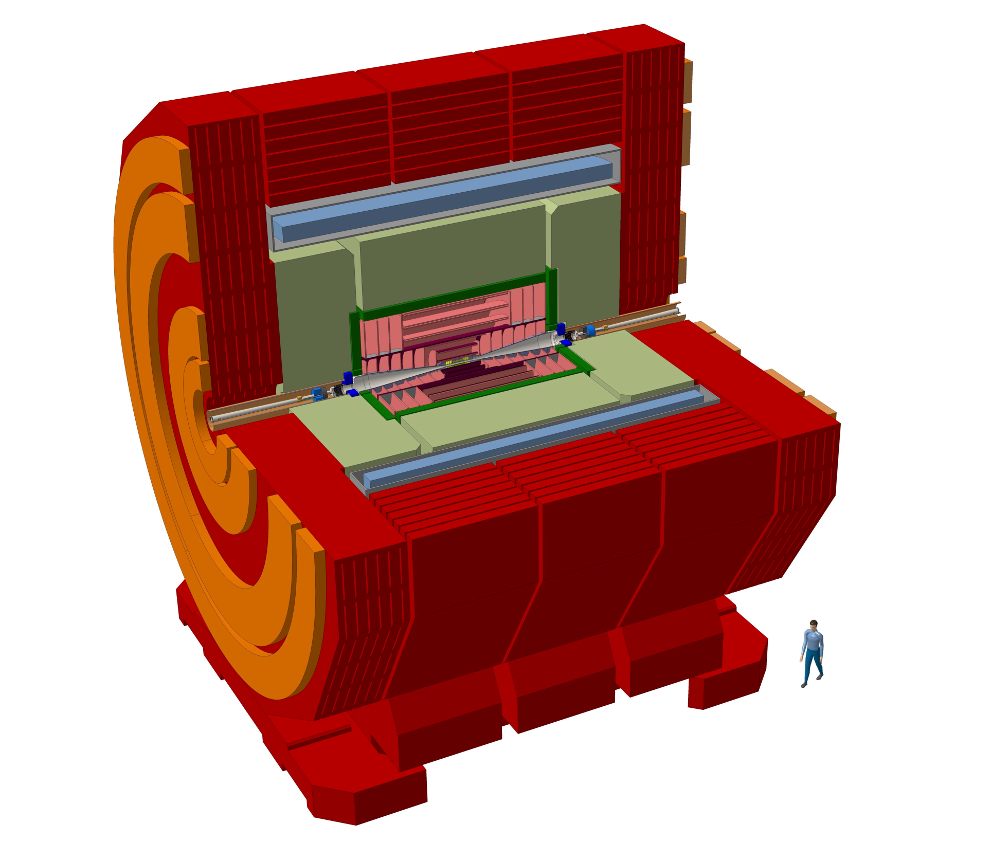
\includegraphics[width=5cm]{other/CLICdp.png}}; 
    
    \node  at (\xRefPosOne+3,\yRefPosOne-2.6) (box){%
      \myCenterBox{\small CLICdet model}
    }; 

\node [myBox, anchor=north east] at (11.-0,\yRefPosOne) (box){%
    \begin{minipage}{0.45\textwidth}
        \begin{itemize}
         \item Future Circular Collider ($e^-e^+$)
%          \item 4 energy stages: $Z$, $WW$, $HZ$, $t\bar{t}$
         \item 4 energy stages: 91 - 365 GeV
         \\ $\to$ thinner calorimeter is sufficient
         \item Bunch spacing: 20 - 3396 ns
        \end{itemize}
    \end{minipage}
};
\node[fancytitle, right=15pt] at (box.north west) {FCC-ee};


\node [PixelBox, anchor=north west] at (\xRefPosOne-5.8,\yRefPosOne-4) (box){%
  \begin{minipage}{0.49\textwidth}
Both experiments demand state-of-the-art detectors with:
         \begin{itemize}
          \item low-material tracking system
           \item precise calorimetery
         \end{itemize}
         
  \end{minipage}
};

% \node [myBox, anchor=north east] at (11.0,-1) (box){%
% \node [anchor=north east] at (\xRefPosOne,\yRefPosOne-4) (box){%
%     \begin{minipage}{0.5\textwidth}
%         \begin{itemize}
%          \item Both experiments demand state-of-the-art detectors with:
%          \begin{itemize}
%           \item low-material tracking system
% %           \item high-granularity calorimeters
%            \item precise calorimetery
%          \end{itemize}
% 
%         \end{itemize}
%     \end{minipage}
% };
% \node[fancytitle, right=15pt] at (box.north west) {Search for $\PWprime$};

  

 
%% HELPER draw advanced helping grid with axises:
% \draw(-0.5,-4) to[grid with coordinates] (11.5,4);

\end{tikzpicture}
\end{frame}
%*****************************************************************************
%*****************************************************************************
\begin{frame}{\large \large Detector constraints from the FCC-ee machine design}
\renewcommand{\yRefPosOne}{0}
\renewcommand{\xRefPosOne}{5.3}
\renewcommand{\xRefIncrementOne}{5.5}

 \begin{tikzpicture}[overlay]
 
  \node[inner sep=0pt] (tmp) at (\xRefPosOne,\yRefPosOne-2.56)
    {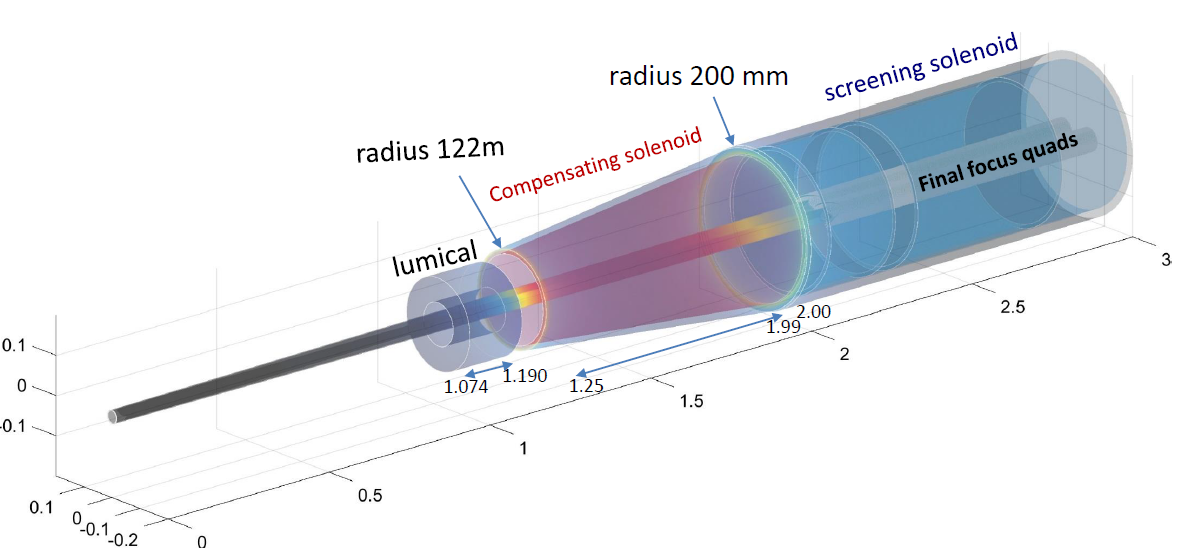
\includegraphics[width=8cm]{other/MDI_lumical.png}};

 
 \node  at (\xRefPosOne,\yRefPosOne+1.5) (box){%
    \begin{minipage}{\textwidth}

  \begin{itemize}
   \item In order to maximize luminosity final focusing quadrupole chosen to be at 2.2 m from IP - {\bf inside the detector}\\[0.2cm]
%    (together with a shielding solenoid)
%    \item To protect the beam from the detector magnetic field an additional compensating solenoid is needed
   \item Compensating solenoid to prevent emittance blow-up from detector magnetic field 
   due to non-zero crossing angle is even closer to the IP \\$\to$ {\bf forward region within 150 mrad is reserved for Machine-Detector Interface} \\[0.2cm]
   \item Constrains {\bf the maximum possible detector magnetic field to 2T} \\(while the CLIC proposal assumes 4T magnetic field)
  \end{itemize}

    \end{minipage}
};

\end{tikzpicture}
 
\end{frame}
%*****************************************************************************
%*****************************************************************************
% \bgroup
% \setbeamercolor{background canvas}{bg=white}
\begin{frame}{}

    \begin{tikzpicture}[overlay]

    %% HELPER draw advanced helping grid with axises:
%     \draw (0,-5) to[grid with coordinates] (11,3);

    \node[right] (textNode) at (3,0) {
      { \large \bf CLD detector layout}
    };
    
    \node[right] (n7) at (4.6,-0.7) {
        \EightStarTaper Tracking system
    };
    
    \node[right] (n8) at (4.6,-1.2) {
        \EightStarTaper Calorimetry
    };

    \node[right] (n9) at (4.6,-1.7) {
        \EightStarTaper The magnet and muon system
    };
    

    
    \tikz[overlay]\draw[thick,black,->] ([xshift=-0.6cm]textNode.south) to [out=270, in=180] ([xshift=-0.1pt]n7.west);
    \tikz[overlay]\draw[thick,black,->] ([xshift=-1.1cm]textNode.south) to [out=270, in=180] ([xshift=-0.1pt]n8.west);
    \tikz[overlay]\draw[thick,black,->] ([xshift=-1.6cm]textNode.south) to [out=270, in=180] ([xshift=-0.1pt]n9.west);    

    \end{tikzpicture}

\end{frame}
% \egroup
%*****************************************************************************
%*****************************************************************************
\begin{frame}{\large \large CLD detector layout}

\renewcommand{\yRefPosOne}{0}
\renewcommand{\xRefPosOne}{5.5}
\renewcommand{\xRefIncrementOne}{5.5}
\begin{tikzpicture}[overlay]

 \node[inner sep=0pt] (tmp) at (\xRefPosOne-2.15,\yRefPosOne-0.56)
    {\includegraphics[width=7.8cm]{other/CLIC_FCC_Top_QuarterView_withLabes.png}};

\node  at (\xRefPosOne,\yRefPosOne+2.8) (box){%
\myCenterBox{\small CLD model}
}; 
    
    \draw[black, thick, ->] (-0.58,-4.76)--(-0.58,3.7) node[pos=0.97, right]{\small R [m]};
    \draw[black, thick, ->] (-0.58,-4.76)--(6.7,-4.76) node[pos=1.02, below]{\small Z [m]};

   \node[inner sep=0pt] (tmp) at (\xRefPosOne-6.28,\yRefPosOne-1.95)
    {2.1};   

  \node[inner sep=0pt] (tmp) at (\xRefPosOne-6.29,\yRefPosOne-0.05)
    {3.5};   

  \node[inner sep=0pt] (tmp) at (\xRefPosOne-6.29,\yRefPosOne+0.95)
    {4.2};   
    
  \node[inner sep=0pt] (tmp) at (\xRefPosOne-6.29,\yRefPosOne+3.2)
    {6.0};   
    
  \node[inner sep=0pt] (tmp) at (\xRefPosOne-3.05,\yRefPosOne-4.9)
    {2.3};   
  \node[inner sep=0pt] (tmp) at (\xRefPosOne-1.14,\yRefPosOne-4.9)
    {3.7};  
  \node[inner sep=0pt] (tmp) at (\xRefPosOne+0.84,\yRefPosOne-4.9)
    {5.4}; 
    
%     \node [PixelBox] at (\xRefPosOne+3.7,\yRefPosOne-4) (box){%
%   \begin{minipage}{0.43\textwidth}
%     Detector design inspired by detectors for CLIC and ILC and optimized for FCC-ee conditions
%   \end{minipage}
% };

% \node [PixelBox] at (\xRefPosOne+3.7,\yRefPosOne+2.5) (box){%
%   \begin{minipage}{0.43\textwidth}
%     CLD detector model is inspired by detectors for CLIC and ILC and optimized for FCC-ee conditions
%   \end{minipage}
% };

\node  at (\xRefPosOne+3.5,\yRefPosOne-0.6) (box){%
    \begin{minipage}{0.5\textwidth}

  \begin{itemize}
      \item Full silicon tracking system - provides $\geqslant$12 hits per track \\[0.6cm]
%       \item 2 T magnetic field (constraints from the machine) $\to$ 2.1 m large tracker radius \\[0.4cm]
      \item Fine-grained ECAL and HCAL optimised for particle flow reconstruction \\[0.6cm]
      \item Superconducting solenoid is outside of the calorimeter \\[0.6cm]
      \item Steel return yoke with muon chambers\\[0.6cm]
   
   \item Forward detector region ($<$ 150 mrad) is reserved for Machine-Detector Interface (accommodates LumiCal)\\[0.6cm]
   
   \item Support structures, cables and services are included in the model
%    : \\ MDI region 
%    (accommodates LumiCal)
   \\[0.3cm]
  \end{itemize}

    \end{minipage}
};







% \node [PixelBox] at (\xRefPosOne+3.7,\yRefPosOne-4) (box){%
%   \begin{minipage}{0.43\textwidth}
%     Detector design inspired by detectors for CLIC and ILC and optimized for FCC-ee conditions
%   \end{minipage}
% };

%% HELPER draw advanced helping grid with axises:
% \draw(-0.5,-4) to[grid with coordinates] (11.5,4);
\end{tikzpicture}

 
\end{frame}
%*****************************************************************************
%*****************************************************************************
\begin{frame}{\large \large Tracking system}

\renewcommand{\yRefPosOne}{0}
\renewcommand{\xRefPosOne}{5.3}
\renewcommand{\xRefIncrementOne}{5.5}
\begin{tikzpicture}[overlay]

\node[PixelBox] (tmp) at  (\xRefPosOne-3.2,\yRefPosOne+1.5) (box){%

  \begin{minipage}{0.46\textwidth}
    \begin{itemize}
     \item Silicon pixels: 25x25$\upmu$m$^2$
     \item Single-point resolution: 3 $\upmu$m
     \item 3 double layers in barrel: \\r = 17, 37, 57 mm
     \item 3 double endcap disks per side: \\ z = 160, 230, 300 mm
     \item Material budget: 0.6$\%$ X$_0$ per double layer
    \end{itemize}

  \end{minipage}
};
\node[fancytitle, right=15pt] at (box.north west) {Vertex detector};

\node[TRTBox] (tmp) at  (\xRefPosOne-3.2,\yRefPosOne-2.7) (box){%

  \begin{minipage}{0.46\textwidth}
    \begin{itemize}
     \item Silicon pixel and microstrips detector
     \item Inner Tracker:
     \begin{itemize}
      \item 3 barrel layers, 7 disks per side
     \end{itemize}
     \item Outer Tracker:
     \begin{itemize}
      \item 3 barrel layers, 4 disks per side
     \end{itemize}
     \item Single-point resolution:
     \begin{itemize}
      \item 7 $\upmu$m x 90 $\upmu$m
      \item except 1st IT disk: 5 $\upmu$m x 5 $\upmu$m
     \end{itemize}
     \item Material:  1.1-1.6$\%$ X$_0$ per layer
%      \item Material budget: 
%      \begin{itemize}
%       \item barrel: 1.1-1.2$\%$ X$_0$ per layer
%       \item disks: 1.4-1.6$\%$ X$_0$ per layer
%      \end{itemize}

     
    \end{itemize}

  \end{minipage}
};
\node[fancytitle, right=15pt] at (box.north west) {Tracker detector};

% \node[PixelBox, inner sep=2pt] (tmp) at  (\xRefPosOne+2,\yRefPosOne+1.3) (box){%
\node[inner sep=0pt] (tmp) at  (\xRefPosOne+2.8,\yRefPosOne-3.1) (box){%
% \node[inner sep=0pt] (tmp) at  (\xRefPosOne+2.5,\yRefPosOne+1.3) (box){%
    {\includegraphics[width=5cm]{other/Sasha_17Jan2018_materialBudget_FCCee_o1_v02.pdf}}
};
% \node[fancytitle, right=5pt] at (box.north west) {VTX + Tracker + Beampipe Material Budget};
    
\node (tmp.west) at  (\xRefPosOne+3.9,\yRefPosOne-4.0) (box){%
  \begin{minipage}{0.44\textwidth}
   VTX + Tracker + Beampipe \\Material Budget
  \end{minipage}
};
    
\node[inner sep=0pt] (tmp) at  (\xRefPosOne+3.0,\yRefPosOne+1.3) (box){%
% \node[inner sep=0pt] (tmp) at  (\xRefPosOne+2.8,\yRefPosOne-2.6) (box){%
    {\includegraphics[width=5cm]{other/full_Tracker_FCCee_probe_v2.pdf}}
};

% \node[TRTBox] (tmp.west) at  (\xRefPosOne-3.2,\yRefPosOne-2.3) (box){%
% 
%   \begin{minipage}{0.46\textwidth}
%    fds dsf 
%   \end{minipage}
% };
    
%     \node  at (\xRefPosOne-2.7,\yRefPosOne-4.7) (box){%
%       \myCenterBox{\small Support structures, cables and services are included}
%     };     
    
% \node  (tmp.west) at (\xRefPosOne-0.5,\yRefPosOne-4.7) (box){%
%     \begin{minipage}{\textwidth}
% 
%     {
%     Support structures, cables and services are included
%     }
% %   \begin{itemize}
% %    \item ???
% % \end{itemize}
% 
%     \end{minipage}
% };
    
    
%% HELPER draw advanced helping grid with axises:
% \draw(-0.5,-4) to[grid with coordinates] (11.5,4);  
\end{tikzpicture}

 
\end{frame}
%*****************************************************************************
%*****************************************************************************
\begin{frame}{\large \large Calorimetry}

\renewcommand{\yRefPosOne}{0}
\renewcommand{\xRefPosOne}{5.3}
\renewcommand{\xRefIncrementOne}{5.5}
\begin{tikzpicture}[overlay]

\node[inner sep=0pt] (tmp) at  (\xRefPosOne-2.9,\yRefPosOne-3.4) (box){%
    {\includegraphics[width=4cm]{other/Sasha_15Mar2018_nuclearInteractionLengthsCalorimeter_FCCee_o1_v02.pdf}}
};

\node[inner sep=0pt] (tmp) at  (\xRefPosOne+3.4,\yRefPosOne-0.5) (box){%
    {\includegraphics[width=7cm]{other/calo_overall_view.pdf}}
};




% \node[TRTBox, inner sep=7pt] (tmp) at  (\xRefPosOne-3.1,\yRefPosOne-3.8) (box){%
%     {\includegraphics[width=5.5cm]{other/HCAL_schematicDrawning.pdf}}
% };
% \node[fancytitle, right=15pt] at (box.north west) {HCAL layer layout};

\node[PixelBox] (tmp) at  (\xRefPosOne-3.2,\yRefPosOne+2.2) (box){%

  \begin{minipage}{0.48\textwidth}
    \begin{itemize}
        \item Si-W sampling calorimeter
        \item cell size 5x5 mm$^2$
        \item 40 layers (1.9 mm thick W plates)
        \item Depth: 22 X$_0$, 1 $\lambda_I$, 20 cm
    \end{itemize}

  \end{minipage}
};
\node[fancytitle, right=15pt] at (box.north west) {Electromagnetic Calorimeter};

\node[TRTBox] (tmp) at  (\xRefPosOne-3.2,\yRefPosOne-0.5) (box){%

  \begin{minipage}{0.48\textwidth}
    \begin{itemize}
        \item Scintillator-steel sampling calorimeter
        \item cell size 30x30 mm$^2$
        \item 44 layers (19 mm thick steel plates)
        \item Depth: 5.5 $\lambda_I$, 117 cm {\small (inspired by ILD)}
    \end{itemize}

  \end{minipage}
};
\node[fancytitle, right=15pt] at (box.north west) {Hadronic Calorimeter};


%% HELPER draw advanced helping grid with axises:
% \draw(-0.5,-4) to[grid with coordinates] (11.5,4);
\end{tikzpicture}

 
\end{frame}
%*****************************************************************************
%*****************************************************************************
\begin{frame}{\large \large The magnet and muon system}

\renewcommand{\yRefPosOne}{0}
\renewcommand{\xRefPosOne}{5.3}
\renewcommand{\xRefIncrementOne}{5.5}
\begin{tikzpicture}[overlay]

\node[inner sep=0pt] (tmp) at  (\xRefPosOne+2.8,\yRefPosOne-0.6) (box){%
    {\includegraphics[width=7cm]{other/FCC_clic_muons.pdf}}
};

\node[PixelBox] (tmp) at  (\xRefPosOne-3.2,\yRefPosOne+1.0) (box){%

  \begin{minipage}{0.5\textwidth}
      \begin{itemize}
     \item Superconducting coil outside calorimeter (90 mm aluminium thick coil)
     \item Return yoke (1.5 m thick steel)
%       \item The simulation model assumes a 2 T homogeneous field in the tracker region, 1 T field in the yoke barrel and no field  in the yoke endcaps
\item The simulation model assumes:
\begin{itemize}
 \item 2 T homogeneous field in the tracker region\\[0.1cm]
 \item 1 T field in the yoke barrel\\[0.1cm]
 \item no field  in the yoke endcaps
\end{itemize}

    \end{itemize}

  \end{minipage}
};
\node[fancytitle, right=15pt] at (box.north west) {The magnet system};

\node[TRTBox] (tmp) at  (\xRefPosOne-3.2,\yRefPosOne-2.6) (box){%

  \begin{minipage}{0.5\textwidth}


    \begin{itemize}
     \item 6 layers of muon chambers (RPC)
     \item Cell size: 30 x 30 mm$^2$
    \end{itemize}
  
  \end{minipage}
};
\node[fancytitle, right=15pt] at (box.north west) {The muon system};

    




%% HELPER draw advanced helping grid with axises:
% \draw(-0.5,-4) to[grid with coordinates] (11.5,4);
\end{tikzpicture}

 
\end{frame}
%*****************************************************************************
%*****************************************************************************
\begin{frame}{\large \large Simulation and reconstruction software tools}

\renewcommand{\yRefPosOne}{0}
\renewcommand{\xRefPosOne}{5.3}
\renewcommand{\xRefIncrementOne}{5.5}
\begin{tikzpicture}[overlay]

%  \node[inner sep=0pt] (tmp) at (\xRefPosOne-2.15,\yRefPosOne-0.56)
%     {\includegraphics[width=7.8cm]{FCCeePictsFromKonrad/CLIC_FCC_Top_QuarterView_withLabes.png}};

    
\node  at (\xRefPosOne,\yRefPosOne) (box){%
    \begin{minipage}{\textwidth}

  \begin{itemize}
   \item For performance study of the CLD detector for FCC-ee 
	 one can benefit from the fully functional and well tested \href{https://github.com/iLCSoft}{\color{blue} iLCSoft} software used by the CLIC and ILC community. \\[0.4cm]
   
   \item Detector geometry description and event simulation: \href{https://github.com/AIDASoft/DD4hep}{\color{blue} DD4hep}
   \item Event Reconstruction: \href{https://github.com/iLCSoft/Marlin}{\color{blue} Marlin}\\[0.4cm]
   
   \item Track Pattern recognition: ConformalTracking
   \item Particle Flow Reconstruction: \href{https://github.com/PandoraPFA}{\color{blue} PandoraPFA} \\[0.6cm]
  
   \item Up-to-date geometry of detector model implemented in lcgeo package: 
   \href{https://github.com/iLCSoft/lcgeo/tree/master/FCCee/compact/FCCee_o1_v02}{\color{blue} FCCee$\_$o1$\_$v02}
%    FCCee$\_$o1$\_$v02

  \end{itemize}

    \end{minipage}
};

\node [PixelBox] at (\xRefPosOne-0.01,\yRefPosOne-3.5) (box){%
  \begin{minipage}{0.99\textwidth}
    Tracking and calorimetry performances have been studied with full detector simulation
  \end{minipage}
};


%% HELPER draw advanced helping grid with axises:
% \draw(-0.5,-4) to[grid with coordinates] (11.5,4);
\end{tikzpicture}

 
\end{frame}
%*****************************************************************************
%*****************************************************************************
% \bgroup
% \setbeamercolor{background canvas}{bg=white}
\begin{frame}{}

    \begin{tikzpicture}[overlay]

    %% HELPER draw advanced helping grid with axises:
%     \draw (0,-5) to[grid with coordinates] (11,3);

    \node[right] (textNode) at (3,0) {
      { \large \bf Tracking performance}
    };
    
    \node[right] (n7) at (4.6,-0.7) {
        \EightStarTaper Momentum and d$_0$ resolutions
    };
    
    \node[right] (n8) at (4.6,-1.2) {
        \EightStarTaper Efficiency for single muons
    };

    \node[right] (n9) at (4.6,-1.7) {
        \EightStarTaper Efficiency in complex events
    };
    
    \tikz[overlay]\draw[thick,black,->] ([xshift=-0.6cm]textNode.south) to [out=270, in=180] ([xshift=-0.1pt]n7.west);
    \tikz[overlay]\draw[thick,black,->] ([xshift=-1.1cm]textNode.south) to [out=270, in=180] ([xshift=-0.1pt]n8.west);
    \tikz[overlay]\draw[thick,black,->] ([xshift=-1.6cm]textNode.south) to [out=270, in=180] ([xshift=-0.1pt]n9.west);    

    \end{tikzpicture}

\end{frame}
% \egroup
%*****************************************************************************
%*****************************************************************************
\begin{frame}{\large \large Momentum and d$_0$ resolutions}
\renewcommand{\yRefPosOne}{-1.5}
\renewcommand{\xRefPosOne}{4.2}
\renewcommand{\xRefIncrementOne}{7.5}
\begin{tikzpicture}[overlay]



 \node[inner sep=0pt] (tmp) at (\xRefPosOne-1.7,\yRefPosOne+0.9)
  {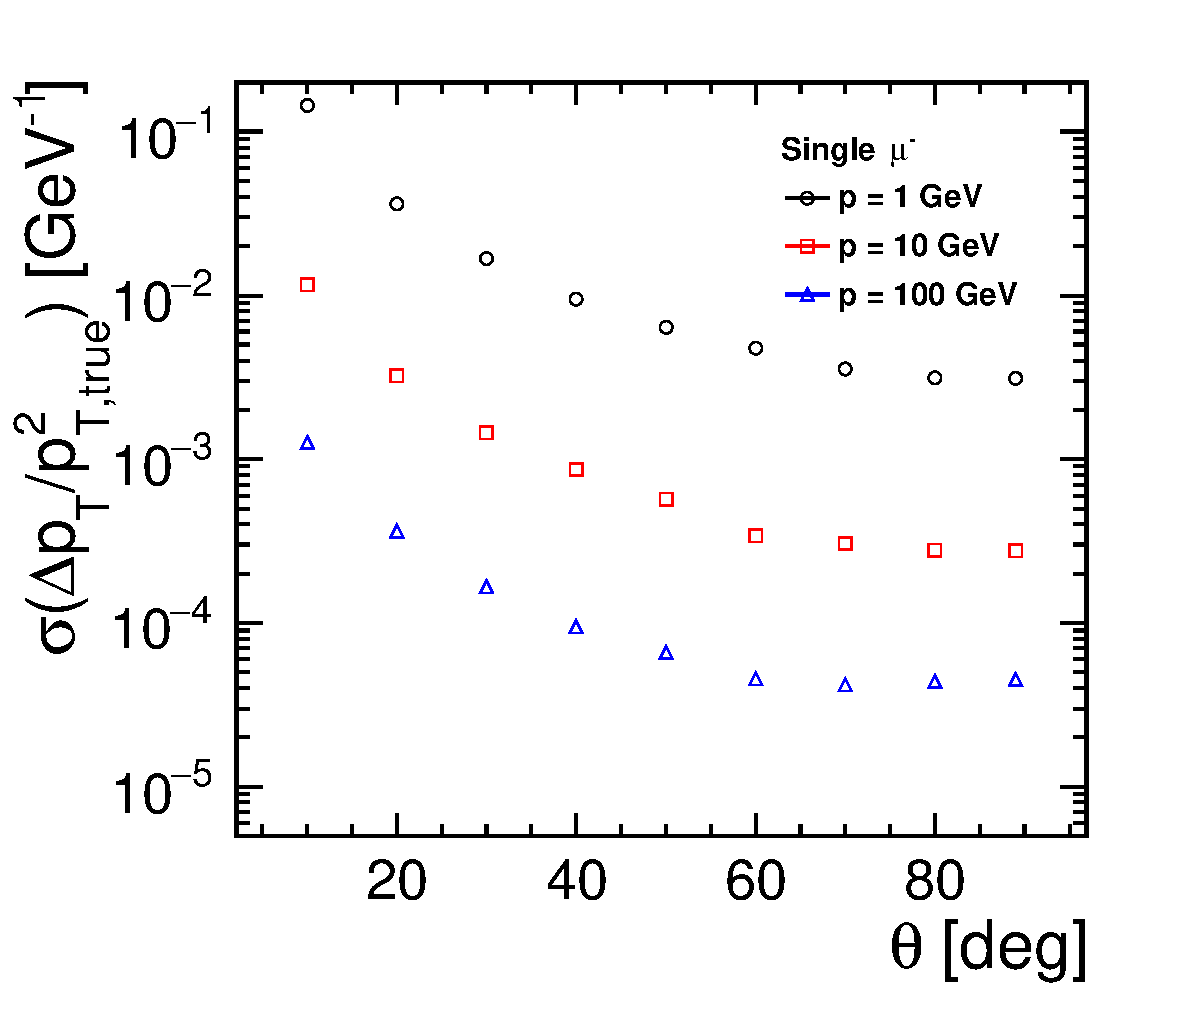
\includegraphics[width=6cm]{fromEmilia/MomRes_vs_theta.pdf}};
  
 \node[inner sep=0pt] (tmp) at (\xRefPosOne+4.5,\yRefPosOne+0.9)
  {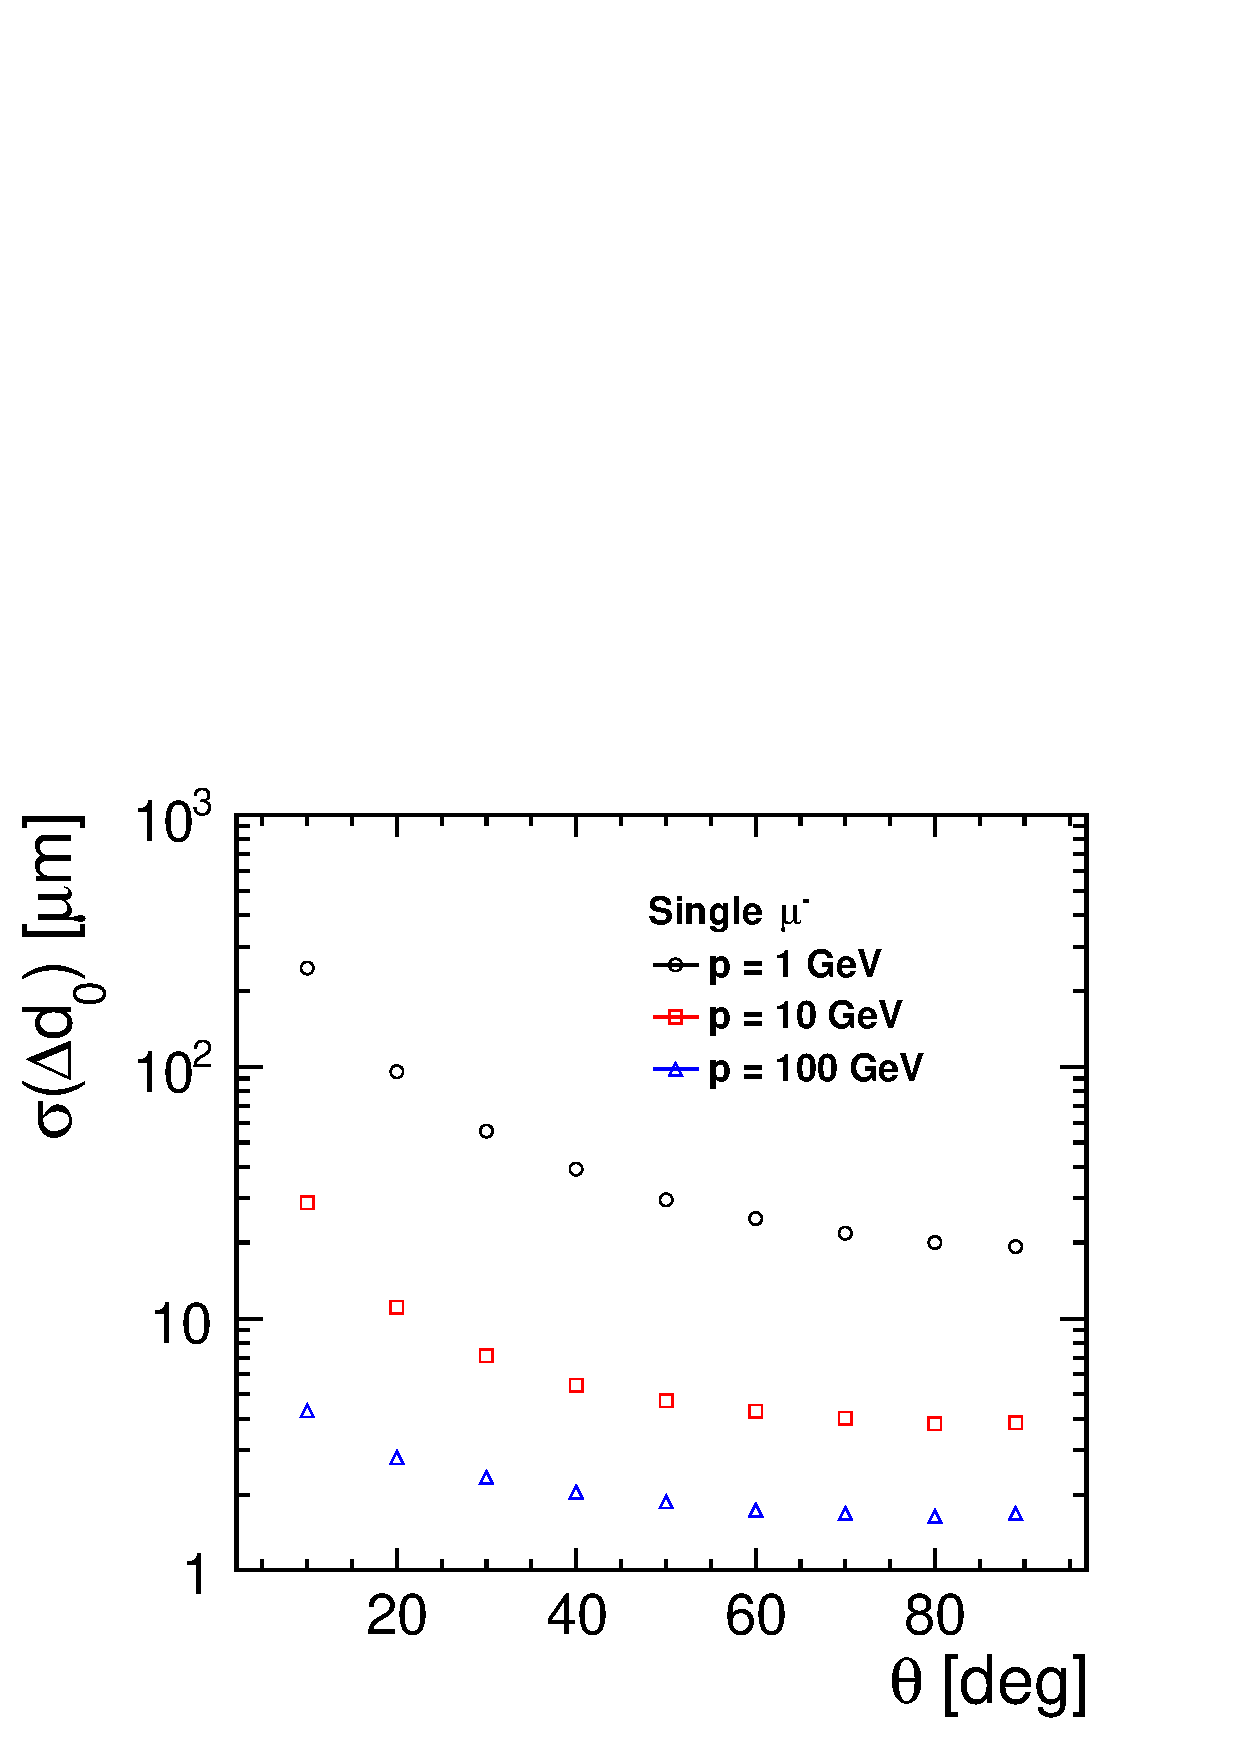
\includegraphics[width=6cm]{fromEmilia/d0Res_vs_theta.pdf}};

 \node[inner sep=0pt] (tmp) at (\xRefPosOne-0.2,\yRefPosOne+3.2)
  {\tiny WORK IN PROGRESS};
 \node[inner sep=0pt] (tmp) at (\xRefPosOne+5.99,\yRefPosOne+3.2)
  {\tiny WORK IN PROGRESS};
  
 \node  at (\xRefPosOne+1,\yRefPosOne+4.5) (box){%
    \begin{minipage}{\textwidth}
      \begin{itemize}
		\item Statistics used: 10k single muons at fixed energy and $\theta$ for each datapoint
      \end{itemize}
    \end{minipage}
  };
  
 \node  at (\xRefPosOne+1,\yRefPosOne-2.5) (box){%
    \begin{minipage}{\textwidth}
      \begin{itemize}
		\item Achieved resolutions for 100 GeV muons in the barrel 
		\begin{itemize}
		 \item momentum resolution: 4x10$^{-5}$ GeV$^{-1}$ 
		 \item transverse impact parameter resolution: $<$ 1$\upmu$m
		\end{itemize}
      \end{itemize}
    \end{minipage}
  };
 
 
 

  
\end{tikzpicture}
\end{frame}
%*****************************************************************************
%*****************************************************************************
\begin{frame}{\large \large Tracking efficiency for single muons}
\renewcommand{\yRefPosOne}{-1.5}
\renewcommand{\xRefPosOne}{4.2}
\renewcommand{\xRefIncrementOne}{7.5}
\begin{tikzpicture}[overlay]

 \node[inner sep=0pt] (tmp) at (\xRefPosOne-1.7,\yRefPosOne+0.9)
  {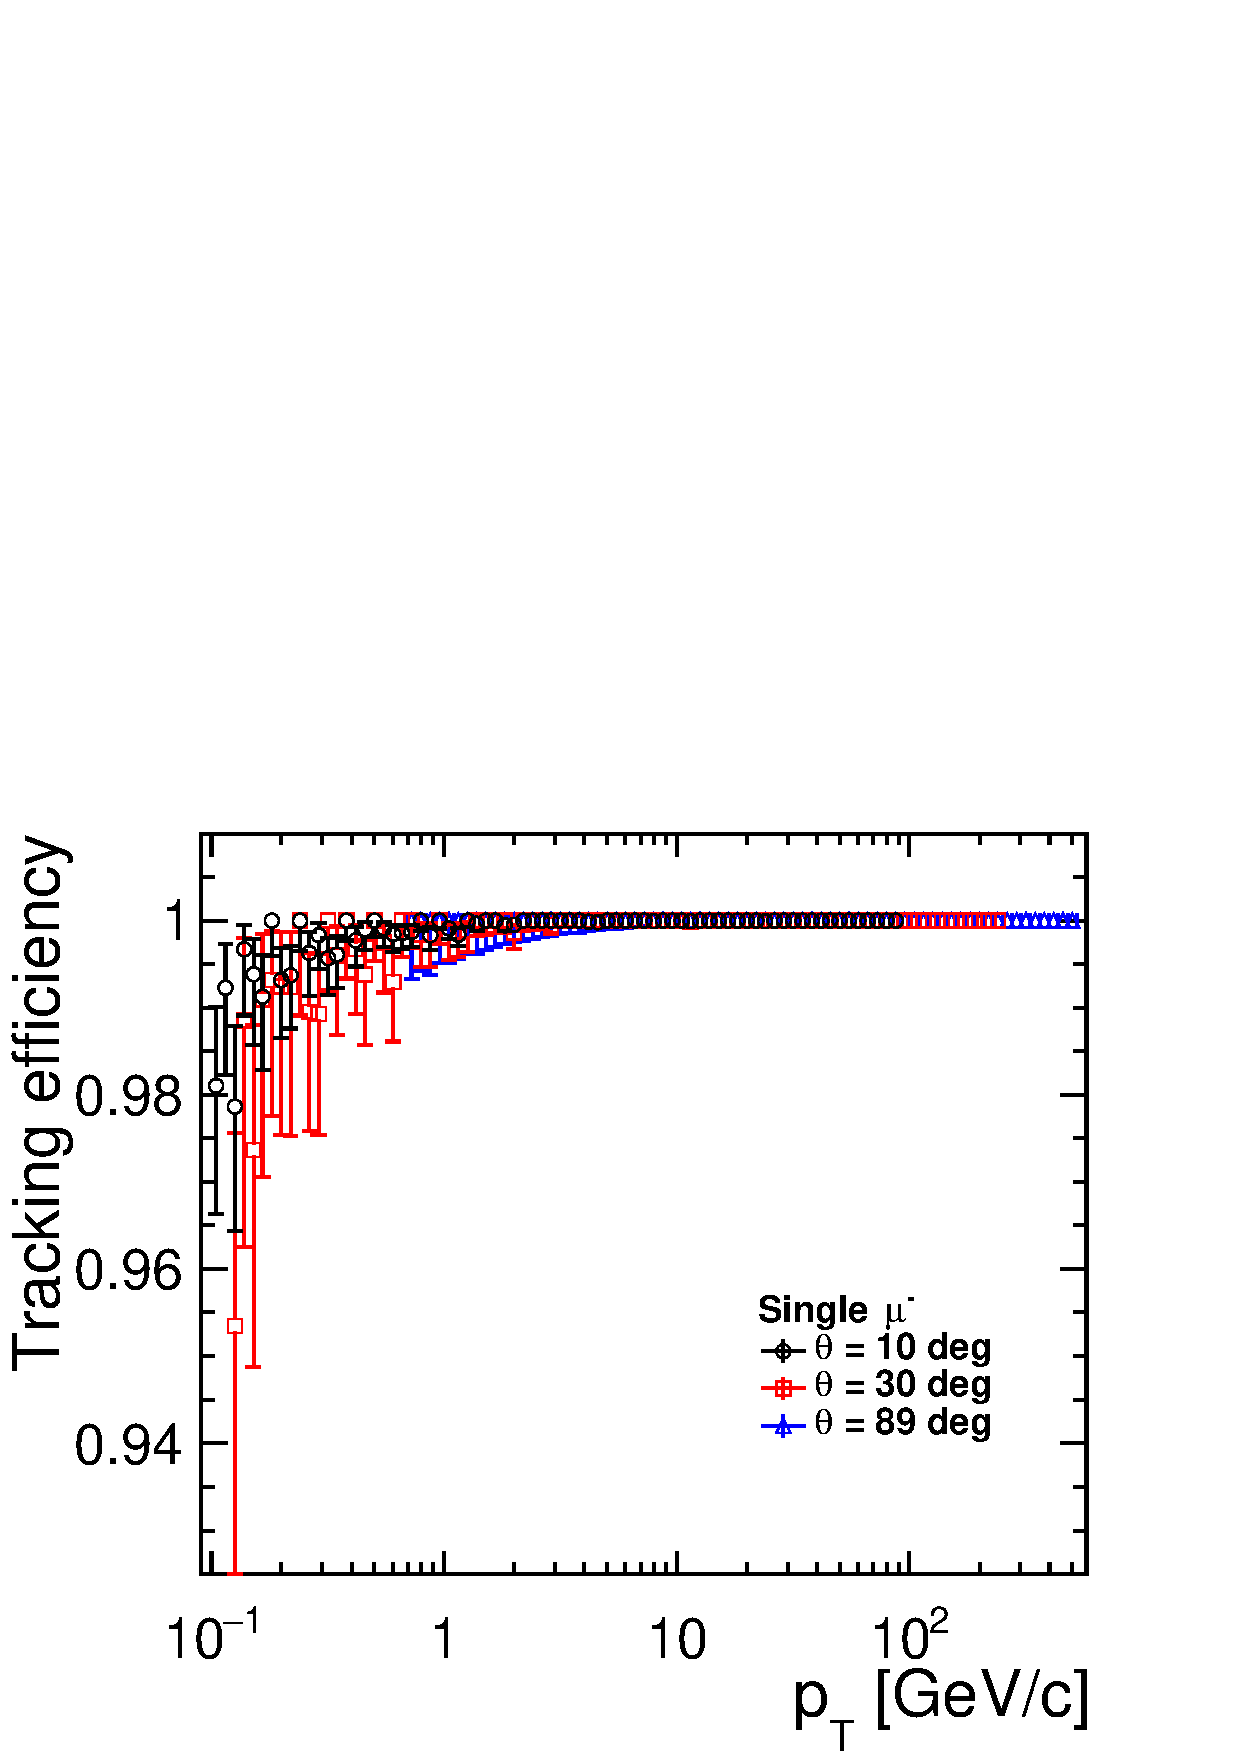
\includegraphics[width=6cm]{fromEmilia/eff_vs_pT.pdf}};
  
 \node[inner sep=0pt] (tmp) at (\xRefPosOne+4.5,\yRefPosOne+0.9)
  {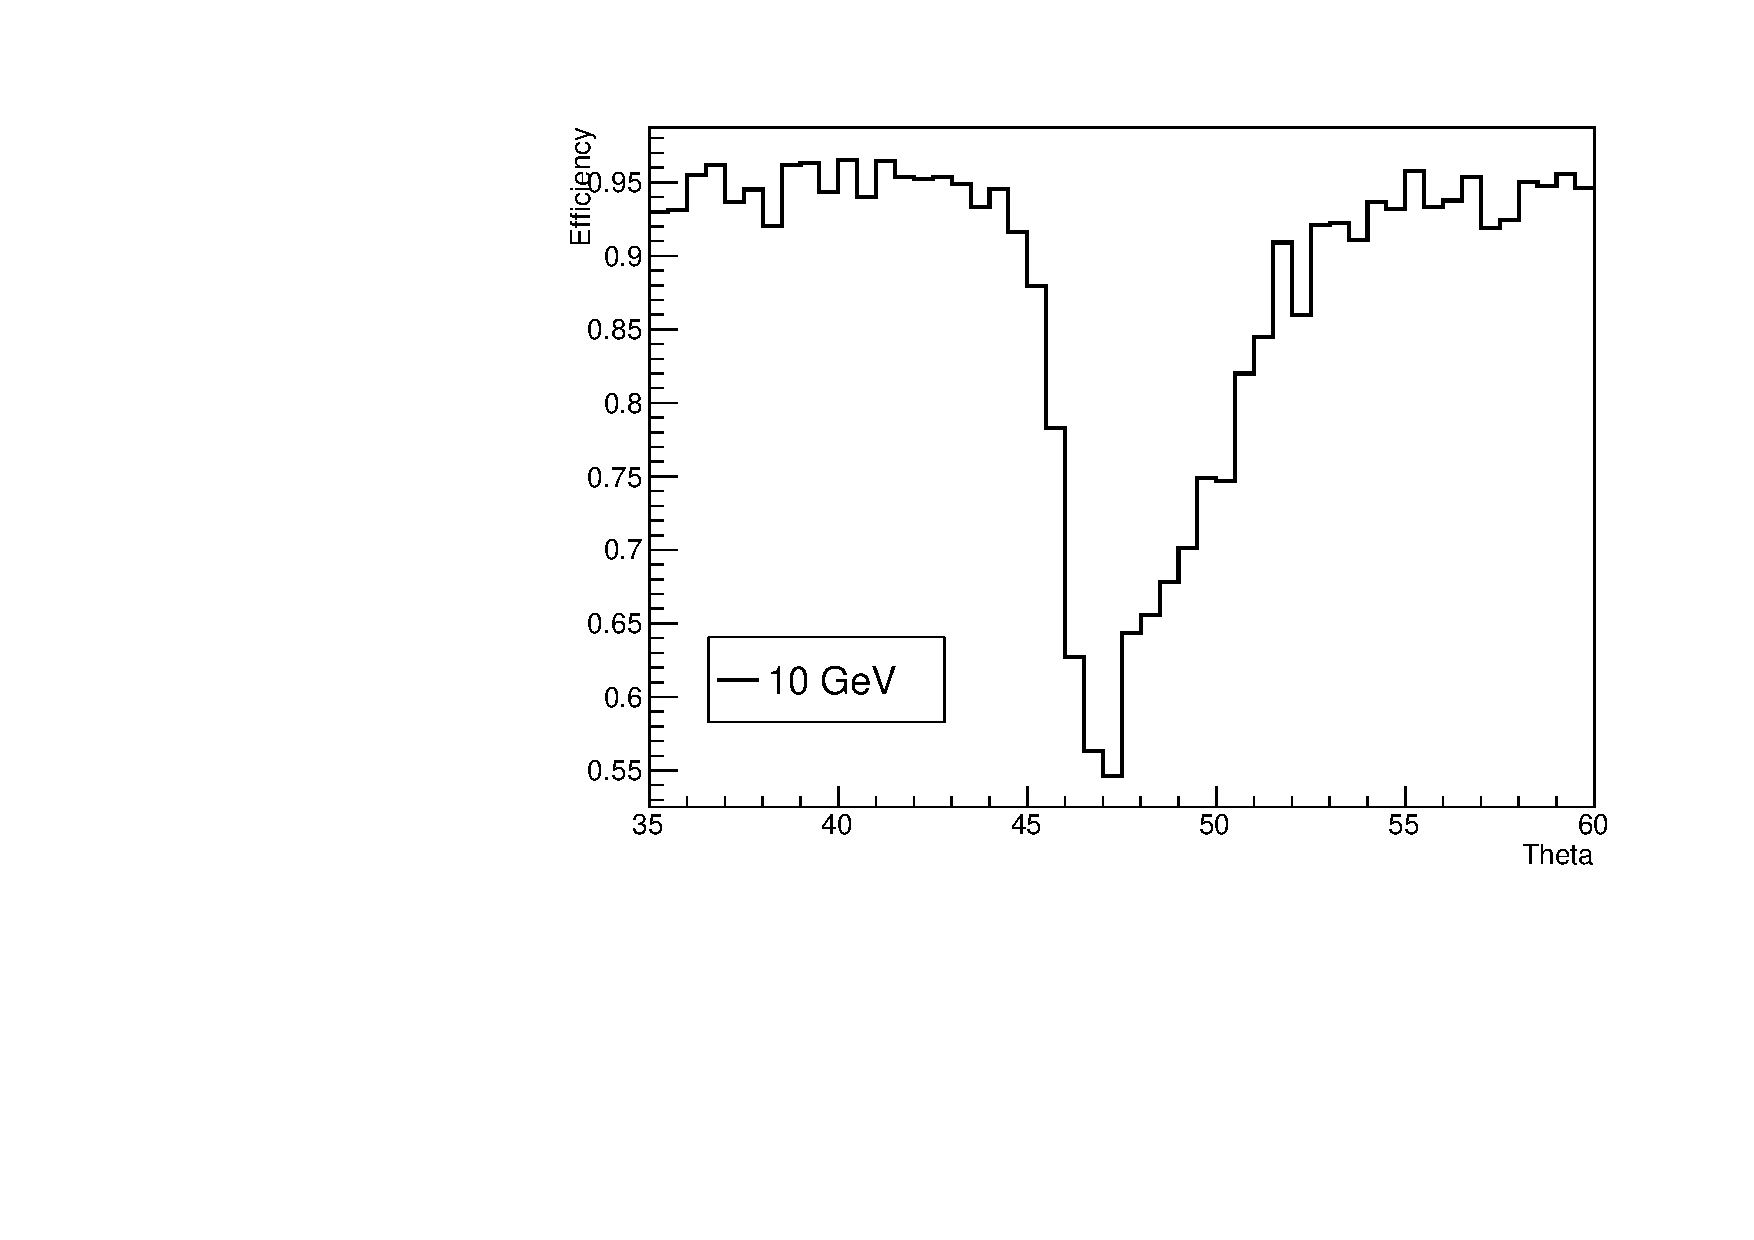
\includegraphics[width=6cm]{fromEmilia/eff_vs_theta.pdf}};

 \node[inner sep=0pt] (tmp) at (\xRefPosOne-0.2,\yRefPosOne+3.2)
  {\tiny WORK IN PROGRESS};
 \node[inner sep=0pt] (tmp) at (\xRefPosOne+5.99,\yRefPosOne+3.2)
  {\tiny WORK IN PROGRESS};
  
   \node  at (\xRefPosOne+1,\yRefPosOne+4.2) (box){%
    \begin{minipage}{1.1\textwidth}
      \begin{itemize}
		\item Efficiency = fraction of reconstructed particles out of the reconstructable MC particles
		\item Reconstructable particles: stable MC particles with $p_T >$ 0.1 GeV/c and $|$cos$(\theta)|<0.99$ which left at least 4 unique hits in tracking system
		\item Statistics used: 2M single muons 
      \end{itemize}
    \end{minipage}
  };
  
 \node  at (\xRefPosOne+1,\yRefPosOne-2.5) (box){%
    \begin{minipage}{\textwidth}
      \begin{itemize}
		\item Fully efficient tracking from 700 MeV over the whole $\theta$ range
      \end{itemize}
    \end{minipage}
  };
 
 \end{tikzpicture}
\end{frame}
%*****************************************************************************
%*****************************************************************************
\begin{frame}{\large \large Tracking efficiency for Z-like boson events decaying at rest into light quarks}
\renewcommand{\yRefPosOne}{-1.5}
\renewcommand{\xRefPosOne}{4.2}
\renewcommand{\xRefIncrementOne}{7.5}
\begin{tikzpicture}[overlay]

 \node[inner sep=0pt] (tmp) at (\xRefPosOne-1.7,\yRefPosOne+0.9)
  {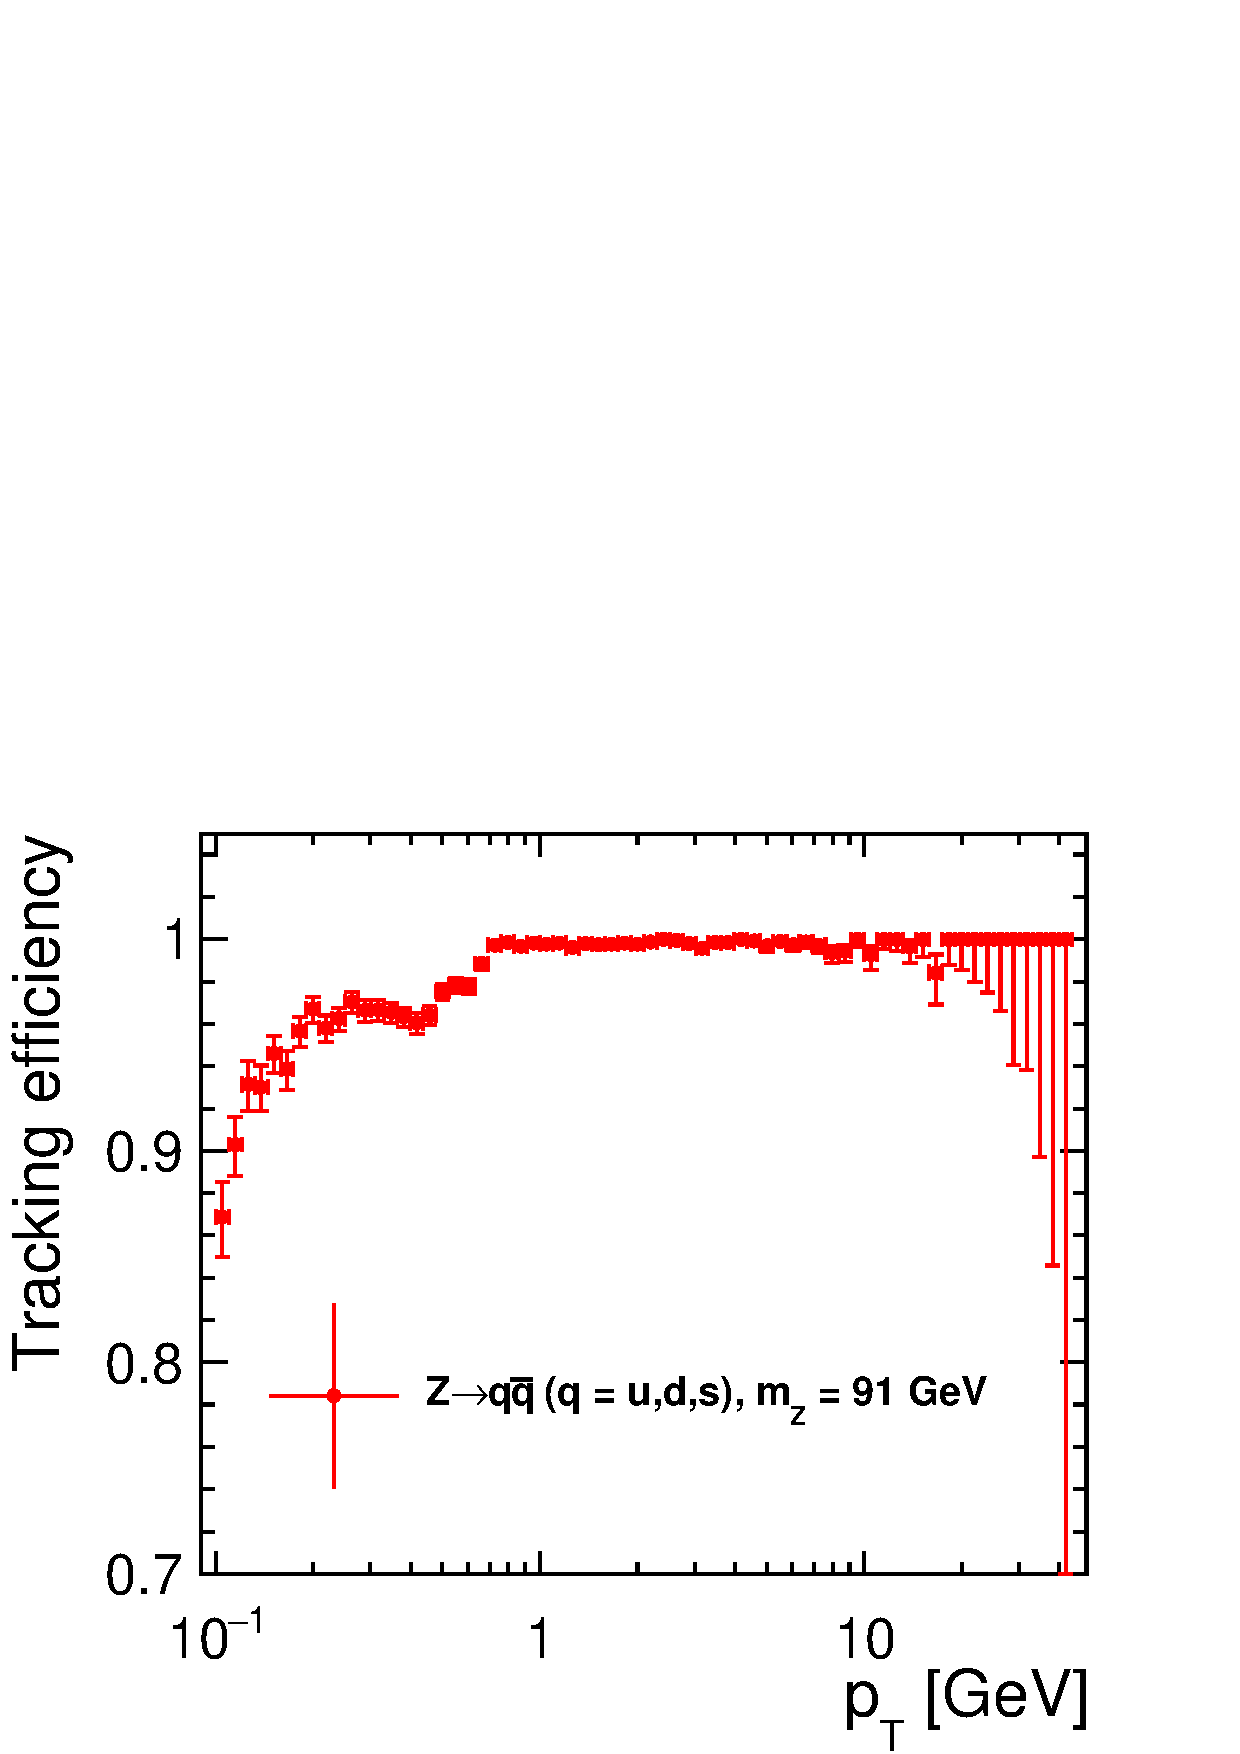
\includegraphics[width=6cm]{fromEmilia/eff_vs_pt_91.pdf}};
  
 \node[inner sep=0pt] (tmp) at (\xRefPosOne+4.5,\yRefPosOne+0.9)
  {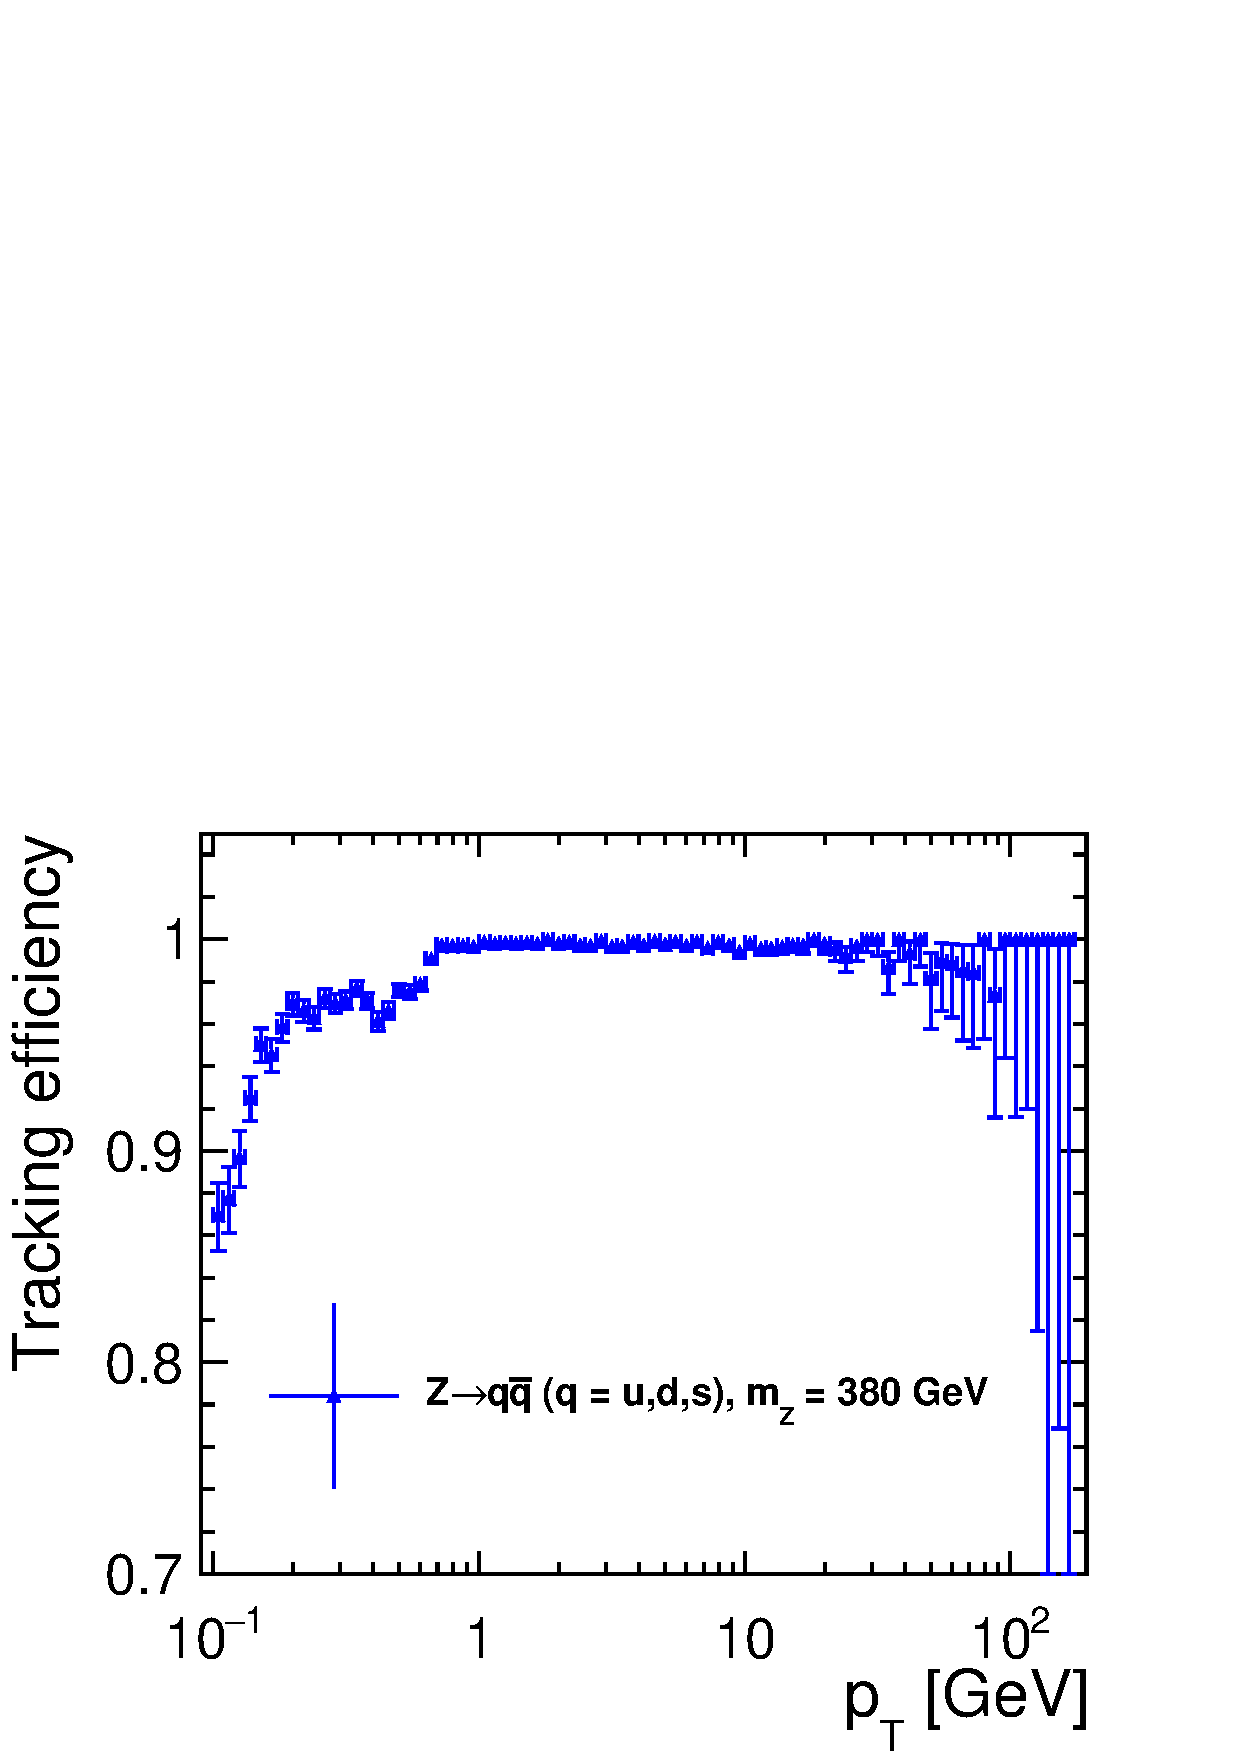
\includegraphics[width=6cm]{fromEmilia/eff_vs_pt_380.pdf}};

 \node[inner sep=0pt] (tmp) at (\xRefPosOne-0.2,\yRefPosOne+3.2)
  {\tiny WORK IN PROGRESS};
 \node[inner sep=0pt] (tmp) at (\xRefPosOne+5.99,\yRefPosOne+3.2)
  {\tiny WORK IN PROGRESS};
  
   \node  at (\xRefPosOne+1,\yRefPosOne+4.2) (box){%
    \begin{minipage}{1.1\textwidth}
      \begin{itemize}
		\item Efficiency = fraction of pure reconstructed particles out of the reconstructable MC particles
		\item Pure reconstructed particles: $\geqslant$75$\%$ of hits from track are associated to the simulated MC particle
      \end{itemize}
    \end{minipage}
  };
  
 \node  at (\xRefPosOne+1,\yRefPosOne-2.5) (box){%
    \begin{minipage}{\textwidth}
      \begin{itemize}
		\item Fully efficient tracking from 700 MeV
      \end{itemize}
    \end{minipage}
  };
  
    \node [TRTBox]  at (\xRefPosOne+4.4,\yRefPosOne-2.35) (box){%
  \begin{minipage}{0.3\textwidth}
   \begin{itemize}
    \item 10 $<\theta<$ 170
    \item vertex R $<$ 50 mm
   \end{itemize}

  \end{minipage}
  };
  \node[fancytitle, right=15pt] at (box.north west) {Selection cuts};
  
 
 \end{tikzpicture}
\end{frame}
%*****************************************************************************

%*****************************************************************************
% \bgroup
% \setbeamercolor{background canvas}{bg=white}
\begin{frame}{}

    \begin{tikzpicture}[overlay]

    %% HELPER draw advanced helping grid with axises:
%     \draw (0,-5) to[grid with coordinates] (11,3);

    \node[right] (textNode) at (3,0) {
      { \large \bf Calorimetry performance}
    };
    
    \node[right] (n7) at (4.8,-0.7) {
        \EightStarTaper Single particle identification efficiency 
    };
    
    \node[right] (n8) at (4.8,-1.2) {
        \EightStarTaper Jet energy resolution
    };

%     \node[right] (n9) at (4.6,-1.7) {
%         \EightStarTaper Tracking efficiency in complex events
%     };
    
    \tikz[overlay]\draw[thick,black,->] ([xshift=-0.8cm]textNode.south) to [out=270, in=180] ([xshift=-0.1pt]n7.west);
    \tikz[overlay]\draw[thick,black,->] ([xshift=-1.3cm]textNode.south) to [out=270, in=180] ([xshift=-0.1pt]n8.west);
%     \tikz[overlay]\draw[thick,black,->] ([xshift=-1.8cm]textNode.south) to [out=270, in=180] ([xshift=-0.1pt]n9.west);    

    \end{tikzpicture}

\end{frame}
% \egroup
%*****************************************************************************
%*****************************************************************************
\begin{frame}{\large \large Single particle identification efficiency}
\renewcommand{\yRefPosOne}{-0.9}
\renewcommand{\xRefPosOne}{4.2}
\renewcommand{\xRefIncrementOne}{7.5}
\begin{tikzpicture}[overlay]

 \node[inner sep=0pt] (tmp) at (\xRefPosOne-1.7,\yRefPosOne-0.6)
%   {\includegraphics[width=6cm]{singleParticleEff/CLD_muon_eff.pdf}};
  {\includegraphics[width=6cm]{singleParticleEff/CLD_muonEff_conformal.pdf}};
  
 \node[inner sep=0pt] (tmp) at (\xRefPosOne+4.5,\yRefPosOne-0.6)
%   {\includegraphics[width=6cm]{singleParticleEff/CLD_pion_eff.pdf}};
  {\includegraphics[width=6cm]{singleParticleEff/CLD_pionEff_conformal.pdf}};


 \node  at (\xRefPosOne+1,\yRefPosOne+3.3) (box){%
    \begin{minipage}{1.1\textwidth}
  \begin{itemize}

   \item Efficiency = fraction of matched reconstructed particles out of the simulated MC particles:
      \begin{itemize}
       \item reconstructed particle of the same type as simulated MC particle
       \item angular matching: $\Delta\theta <$ 1 mrad and $\Delta\phi <$ 2 mrad
       \item energy matching:\\
       - charged particles: $|p_T^{truth} - p_T^{PFO}| < 5\%$ $p_T^{truth} $ \\
       - photons: $\Delta$$E < 5\times\sigma$(ECal) $\approx 0.75\times \sqrt{E}$
      \end{itemize}
    \end{itemize}
    \end{minipage}
  };

  \node [TRTBox]  at (\xRefPosOne+4.8,\yRefPosOne+2.7) (box){%
  \begin{minipage}{0.4\textwidth}
   Sample: single particles with flat cos($\theta$) distribution and fixed energy
  \end{minipage}
  };


  
         \node  at (\xRefPosOne-3.1,\yRefPosOne+1.75) (box){%
    \myCenterBox{\small Muons}
    };     

       \node  at (\xRefPosOne+3,\yRefPosOne+1.75) (box){%
    \myCenterBox{\small Pions}
    };     

 \node[inner sep=0pt] (tmp) at (\xRefPosOne-0.1,\yRefPosOne+1.75)
  {\tiny WORK IN PROGRESS};
 
 \node[inner sep=0pt] (tmp) at (\xRefPosOne+6.1,\yRefPosOne+1.75)
  {\tiny WORK IN PROGRESS};
    
 \node  at (\xRefPosOne+1,\yRefPosOne-3.5) (box){%
    \begin{minipage}{\textwidth}
      \begin{itemize}
        \item $>$99$\%$ muon efficiency and 93-95$\%$ pion efficiency for E$>$10 GeV
        \item Pion inefficiency due to misreconstruction of particle type
      \end{itemize}
    \end{minipage}
  };
 
 \end{tikzpicture}
\end{frame}
%*****************************************************************************
%*****************************************************************************
\begin{frame}{\large \large Single particle identification efficiency}
\renewcommand{\yRefPosOne}{-0.5}
\renewcommand{\xRefPosOne}{4.2}
\renewcommand{\xRefIncrementOne}{7.5}
\begin{tikzpicture}[overlay]

 \node[inner sep=0pt] (tmp) at (\xRefPosOne-1.7,\yRefPosOne-0.6)
  {\includegraphics[width=6cm]{singleParticleEff/CLD_photonEff_conformal}}; 
  
 \node[inner sep=0pt] (tmp) at (\xRefPosOne+4.5,\yRefPosOne-0.6)
  {\includegraphics[width=6cm]{singleParticleEff/CLD_electron_eff.pdf}};


 \node  at (\xRefPosOne+1,\yRefPosOne+2.9) (box){%
    \begin{minipage}{1.1\textwidth}
  \begin{itemize}

   \item Photon merging procedure is used to recover inefficiency due to photon conversion and electron Bremsstrahlung
   \item Pandora parameters were retuned in order to recover some electron inefficiency due to Bremsstrahlung
    \end{itemize}
    \end{minipage}
  };


 \node  at (\xRefPosOne+1,\yRefPosOne-3.5) (box){%
    \begin{minipage}{\textwidth}
      \begin{itemize}
        \item $>95\%$ photons and 93-95 $\%$ electron efficiency for E$>$10 GeV
%         {\tiny [TODO electron plot has to be updated]}
      \end{itemize}
    \end{minipage}
  };
   
       \node  at (\xRefPosOne-3,\yRefPosOne+1.75) (box){%
    \myCenterBox{\small Photons}
    };     

       \node  at (\xRefPosOne+3.25,\yRefPosOne+1.75) (box){%
    \myCenterBox{\small Electrons}
    };     

 \node[inner sep=0pt] (tmp) at (\xRefPosOne-0.1,\yRefPosOne+1.75)
  {\tiny WORK IN PROGRESS};
 
 \node[inner sep=0pt] (tmp) at (\xRefPosOne+6.1,\yRefPosOne+1.75)
  {\tiny WORK IN PROGRESS};
    
 \end{tikzpicture}
\end{frame}
%*****************************************************************************
%*****************************************************************************
\begin{frame}{\large \large Jet Energy Resolution}
\renewcommand{\yRefPosOne}{-0.5}
\renewcommand{\xRefPosOne}{4.2}
\renewcommand{\xRefIncrementOne}{7.5}
\begin{tikzpicture}[overlay]

 \node[inner sep=0pt] (tmp) at (\xRefPosOne-1.7,\yRefPosOne+0.9)
%   {\includegraphics[width=6cm]{/home/oviazlo/Work/Note_FCCeeDetector/figures/Sasha_17Jan2018_jet_energy_res.pdf}};
  {\includegraphics[width=6cm]{JER/jet_energy_res_conformal_apr6.pdf}};
  
 \node[inner sep=0pt] (tmp) at (\xRefPosOne+4.5,\yRefPosOne+0.9)
%   {\includegraphics[width=6cm]{/home/oviazlo/Desktop/beamerPresentations/FCCee/pictures/CEPC_workshop/../oct11_2017/jet_energy.pdf}};
% {\includegraphics[width=6cm]{FCCweek/jet_energy.pdf}};
{\includegraphics[width=6cm]{JER/jet_energy_conformal_apr6.pdf}};

  
 \node[inner sep=0pt] (tmp) at (\xRefPosOne-0.1,\yRefPosOne+3.2)
  {\tiny WORK IN PROGRESS};
 \node[inner sep=0pt] (tmp) at (\xRefPosOne+6.1,\yRefPosOne+3.2)
  {\tiny WORK IN PROGRESS};
  
  
   \node  at (\xRefPosOne+1,\yRefPosOne+3.6) (box){%
    \begin{minipage}{1.1\textwidth}
  \begin{itemize}
   \item Z-like boson events decaying at rest into light quarks (two back-to-back jets)
    \end{itemize}
    \end{minipage}
  };

  
%  \node[inner sep=0pt] (tmp) at (\xRefPosOne+4.5,\yRefPosOne-2.8)
%   {\includegraphics[width=4cm]{/home/oviazlo/Desktop/beamerPresentations/FCCee/pictures/CEPC_workshop/../oct11_2017/jetRes_formula.png}
%   };
%  
%   \node[inner sep=0pt] (tmp) at (\xRefPosOne+4.5,\yRefPosOne-3.7)
%   {\myCenterBox[yellow]{\href{http://arxiv.org/abs/1209.4039}{arXiv:1209.4039}}  };
 
 
  \node [PixelBox, inner sep=4pt]  at (\xRefPosOne+4.7,\yRefPosOne-2.9) (box){%
    \begin{minipage}{0.45\textwidth}
    \small
		Jet energy (E$_j$) is measured as a half of total energy (E$_{jj}$) of Z$\to q\bar{q}$ (q=u,d,s) di-jet event\\
		
		\hspace{0.4cm}
		  {\includegraphics[width=4cm]{other/jetRes_formula.png}}
		
    \end{minipage}
  };
 
 
 \node  at (\xRefPosOne-0.3,\yRefPosOne-2.8) (box){%
    \begin{minipage}{0.8\textwidth}
      \begin{itemize}
		\item Jet energy resolution in barrel region:
        \begin{itemize}
            \item 45.5 GeV jets: 4-4.5 $\%$
            \item 190 GeV jets: 3-4 $\%$ \\ [0.2cm]
        \end{itemize}
        \item Total energy is reconstructed with 1$\%$ accuracy:
        \begin{itemize}
            \item 91 GeV: \hspace{0.07cm} 90.2 GeV
            \item 380 GeV: 377.0 GeV
        \end{itemize}
%         \item comparable resolution with the CLIC detector 

      \end{itemize}
    \end{minipage}
  };
  
\end{tikzpicture}
\end{frame}
%*****************************************************************************
%*****************************************************************************
\begin{frame}{\large \large Summary and Outlook}
 
 \renewcommand{\yRefPosOne}{0} 
\renewcommand{\xRefPosOne}{5.3}
\renewcommand{\xRefIncrementOne}{5.5}
\begin{tikzpicture}[overlay]

       
\node [TRTBox]  at (\xRefPosOne,\yRefPosOne+2) (box){%
  \begin{minipage}{0.99\textwidth}
  
 \begin{itemize}
  \item The CLD detector design for the Conceptual Design Report has been presented
  \item Tracking and calorimetry performance studies with full detector simulation demonstrates excellent overall detector performance 
    \end{itemize}
  \end{minipage}
};
\node[fancytitle, right=15pt] at (box.north west) {Summary};

\node [PixelBox] at (\xRefPosOne,\yRefPosOne-2) (box){%
  \begin{minipage}{0.99\textwidth}
  
\begin{itemize}
 \item Further detector performance simulation studies
 \begin{itemize}
 \item flavour tagging performance  
 \item overlay of incoherent pairs (in progress) and synchrotron radiation backgrounds\\[0.3cm]
%   \item If needed optimize timing and/or p$_T$ cuts to mitigate impact of background\\[0.3cm]
 \end{itemize}
 \item Full simulation studies of different physics processes 
 \begin{itemize}
  \item software framework and detector model available \\[0.3cm]
 \end{itemize}
 \item Engineering studies
 \begin{itemize}
  \item cooling studies of all subdetectors (no power pulsing)
  \item ECAL optimisation (technology choices, number of layers)
  \item detector opening / maintenance scenarios, impact for detector layout 
 \end{itemize}

\end{itemize}

  
%  \begin{itemize}
%   \item Tracking performance
%   \begin{itemize}
%    \item Momentum resolution and track reconstruction efficiency
%   \end{itemize}
%   \item Calorimetry performance
%   \begin{itemize}
%    \item Single particle ID efficiency 
%    \item Jet energy resolution
%   \end{itemize}
%     \end{itemize}
    
  \end{minipage}
};
\node[fancytitle, right=15pt] at (box.north west) {Outlook};

\node[right] (textNode) at (3,-4.5) {
      { \large \bf Thank you for your attention! }
    };

\end{tikzpicture}
  
\end{frame}
%*****************************************************************************
%*****************************************************************************
% \begin{frame}
% \frametitle{Possible additional plots} 
% 
% \renewcommand{\yRefPosOne}{0}
% \renewcommand{\xRefPosOne}{5.3}
% \renewcommand{\xRefIncrementOne}{5.5}
% 
% \begin{tikzpicture}[overlay]
% 
% \node at (\xRefPosOne,\yRefPosOne) (box){%
%   \begin{minipage}{0.99\textwidth}
%    \begin{itemize}
%   \item Tracking performance:
%   \begin{itemize}
%    \item Angular, $d_0$, $z_0$ resolutions
%   \end{itemize}
% 
%   
%   \item Plots with background overlaid: 
%   \begin{itemize}
%    \item tracking efficiency
%    \item signle particle ID efficiency
%    \item jet energy resolution
%   \end{itemize}
% 
%     \end{itemize}
%   \end{minipage}
% };
% 
% %% HELPER draw advanced helping grid with axises:
% % \draw(-0.5,-4) to[grid with coordinates] (11.5,4);
%  
% \end{tikzpicture}
% \end{frame}
%*****************************************************************************
\backupbegin
%*****************************************************************************
\begin{frame}
\frametitle{BACKUP} 
 
\end{frame}
%*****************************************************************************
%*****************************************************************************
\begin{frame}{\large \large CLD vs CLICdet dimensions}
 
\renewcommand{\yRefPosOne}{0}
\renewcommand{\xRefPosOne}{5.3}
\renewcommand{\xRefIncrementOne}{5.5}
\begin{tikzpicture}[overlay]


 \node[TRTBox] (tmp) at (\xRefPosOne,\yRefPosOne-0.5)
  { 
    \begin{minipage}{0.8\textwidth}

    \resizebox{\columnwidth}{!}{%
      \begin{tabular}{lccc}
	 & CLICdet & & CLD \\[0.18cm]
	VTX Barrel & 31-60 mm & $\Longrightarrow$ & 17-59 mm \\[0.18cm]
	VTX Endcap & Spirals & $\Longrightarrow$ & Disks \\[0.18cm]
	Tracker radius & 1486 mm & $\Longrightarrow$ & 2100 mm \\[0.18cm]
% 	ECAL thickness & 202 mm & $\Longrightarrow$ & 202 mm \\[0.18cm]
% 	HCAL thickness & 44 $\times$ 7.5 $\lambda_0$ & $\Longrightarrow$ & 44 $\times$ 5.5 $\lambda_0$ \\[0.18cm]
	ECAL thickness & 40 layers, 22 X$_0$ & $\Longrightarrow$ & 40 layers, 22 X$_0$ \\[0.18cm]
	HCAL thickness & 60 layers, 7.5 $\lambda_I$ & $\Longrightarrow$ & 44 layers, 5.5 $\lambda_I$ \\[0.18cm]
	Yoke thickness & 1989 mm & $\Longrightarrow$ & 1521 mm \\[0.18cm]
	MDI (forward region) &  & $\Longrightarrow$ & $<$ 150 mrad \\[0.4cm]
	Solenoid field & 4 Tesla & $\Longrightarrow$ & 2 Tesla \\
	
      \end{tabular}%
    }
    \end{minipage}
  };
  


\node at (\xRefPosOne,\yRefPosOne+2.6) (box){%
\myCenterBox[TRTColor]{Overall dimensions of CLIC and FCC-ee detectors}
};
  
\end{tikzpicture}
\end{frame}
%*****************************************************************************
%*****************************************************************************
\begin{frame}{\large \large Pion identification efficiency}
\renewcommand{\yRefPosOne}{-0.5}
\renewcommand{\xRefPosOne}{4.2}
\renewcommand{\xRefIncrementOne}{7.5}
\begin{tikzpicture}[overlay]

 \node[inner sep=0pt] (tmp) at (\xRefPosOne-1.7,\yRefPosOne-0.6)
  {\includegraphics[width=6cm]{singleParticleEff/pion_eff_vs_theta_E20.pdf}}; 
  
 \node[inner sep=0pt] (tmp) at (\xRefPosOne+4.5,\yRefPosOne-0.6)
  {\includegraphics[width=6cm]{singleParticleEff/pion_eff_vs_theta_E100.pdf}};


 \node  at (\xRefPosOne+1,\yRefPosOne+2.9) (box){%
    \begin{minipage}{1.1\textwidth}
  \begin{itemize}

   \item Pion ID efficiency and inefficiency as function of cos($\theta$)
    \end{itemize}
    \end{minipage}
  };


 \node  at (\xRefPosOne+1,\yRefPosOne-3.5) (box){%
    \begin{minipage}{\textwidth}
      \begin{itemize}
        \item High momentum pions more often are misreconstructed as muons in barrel
      \end{itemize}
    \end{minipage}
  };
   
       \node  at (\xRefPosOne-2.65,\yRefPosOne+1.75) (box){%
    \myCenterBox{\small 20 GeV pions}
    };     

       \node  at (\xRefPosOne+3.6,\yRefPosOne+1.75) (box){%
    \myCenterBox{\small 100 GeV pions}
    };     

 \node[inner sep=0pt] (tmp) at (\xRefPosOne-0.1,\yRefPosOne+1.75)
  {\tiny WORK IN PROGRESS};
 
 \node[inner sep=0pt] (tmp) at (\xRefPosOne+6.1,\yRefPosOne+1.75)
  {\tiny WORK IN PROGRESS};
    
 \end{tikzpicture}
\end{frame}
%*****************************************************************************
%*****************************************************************************
\begin{frame}{\large \large Electron identification efficiency}
\renewcommand{\yRefPosOne}{-0.5}
\renewcommand{\xRefPosOne}{4.2}
\renewcommand{\xRefIncrementOne}{7.5}
\begin{tikzpicture}[overlay]

 \node[inner sep=0pt] (tmp) at (\xRefPosOne-1.7,\yRefPosOne-0.6)
  {\includegraphics[width=6cm]{singleParticleEff/electron_eff_vs_theta_E20.pdf}}; 
  
 \node[inner sep=0pt] (tmp) at (\xRefPosOne+4.5,\yRefPosOne-0.6)
  {\includegraphics[width=6cm]{singleParticleEff/electron_eff_vs_theta_E100.pdf}};


 \node  at (\xRefPosOne+1,\yRefPosOne+2.9) (box){%
    \begin{minipage}{1.1\textwidth}
  \begin{itemize}

   \item Electron ID efficiency and inefficiency as function of cos($\theta$)
    \end{itemize}
    \end{minipage}
  };


 \node  at (\xRefPosOne+1,\yRefPosOne-3.5) (box){%
    \begin{minipage}{\textwidth}
      \begin{itemize}
        \item Inefficiency for high-momentum electrons can be recovered by better Bremsstrahlung recovery algorithm
      \end{itemize}
    \end{minipage}
  };
   
       \node  at (\xRefPosOne-2.5,\yRefPosOne+1.75) (box){%
    \myCenterBox{\small 20 GeV electrons}
    };     

       \node  at (\xRefPosOne+3.75,\yRefPosOne+1.75) (box){%
    \myCenterBox{\small 100 GeV electrons}
    };     

 \node[inner sep=0pt] (tmp) at (\xRefPosOne-0.1,\yRefPosOne+1.75)
  {\tiny WORK IN PROGRESS};
 
 \node[inner sep=0pt] (tmp) at (\xRefPosOne+6.1,\yRefPosOne+1.75)
  {\tiny WORK IN PROGRESS};
    
 \end{tikzpicture}
\end{frame}
%*****************************************************************************
%*****************************************************************************
\begin{frame}{\large \large Electron identification efficiency (Pandora track-cluster association algorithm)}

\renewcommand{\yRefPosOne}{-0.5}
\renewcommand{\xRefPosOne}{5.5}
\renewcommand{\xRefIncrementOne}{5.5}
\begin{tikzpicture}[overlay]

 \node[inner sep=0pt] (tmp) at (\xRefPosOne-3,\yRefPosOne+1.2)
    {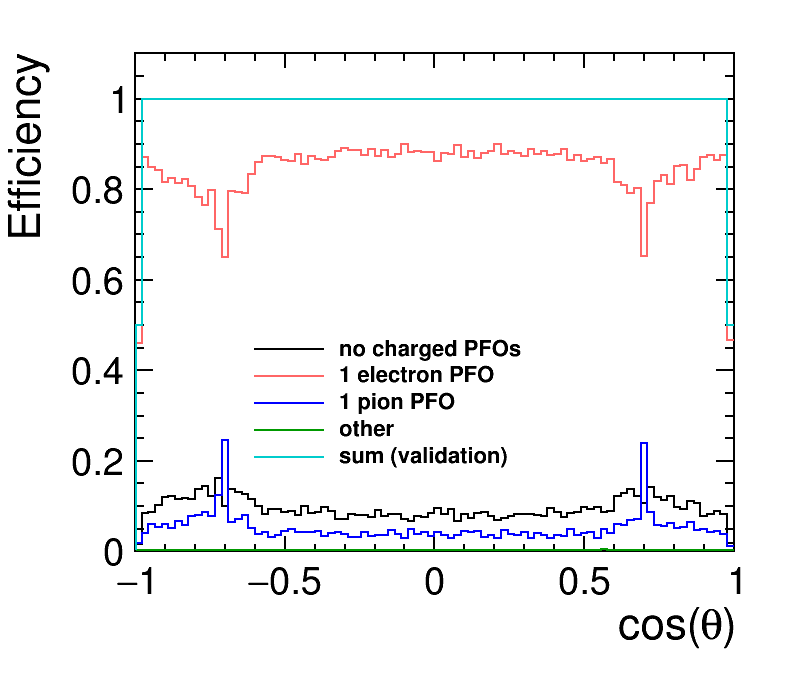
\includegraphics[width=6.2cm]{other/calice_CLIC_vs_FCCee_effVsTheta_fakes_electrons_E10.pdf}};
    
 \node[inner sep=0pt] (tmp) at (\xRefPosOne+3,\yRefPosOne-0.1)
    {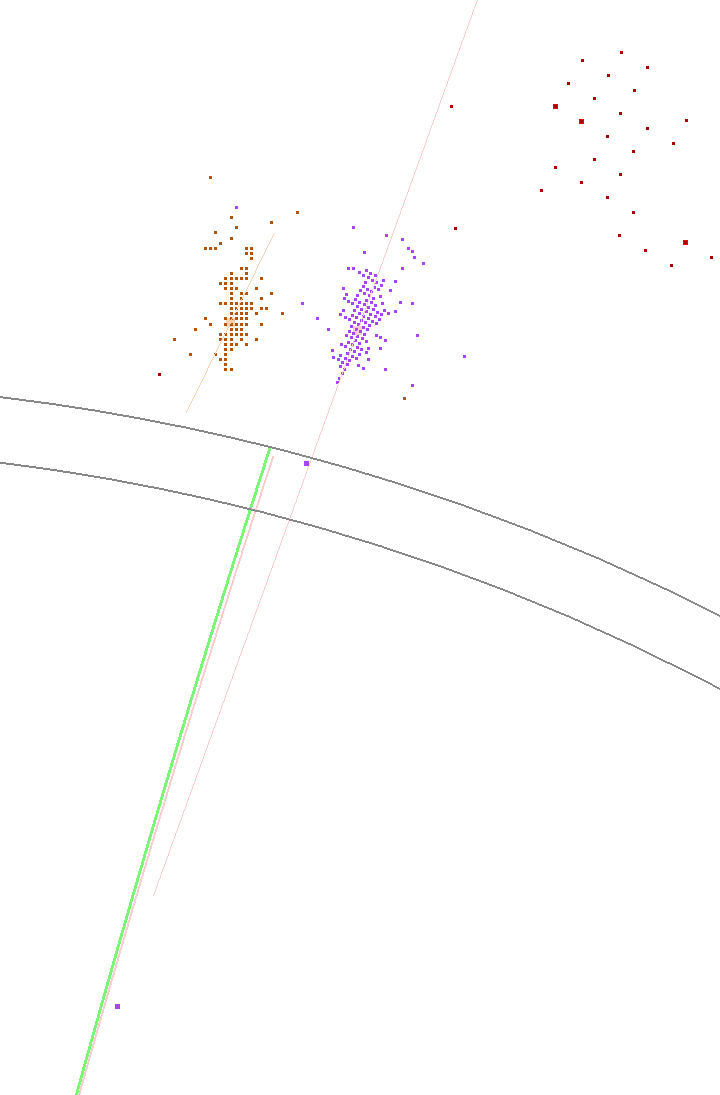
\includegraphics[width=5.5cm]{other/eventDisplay.png}};
    
    \node  at (\xRefPosOne-1.5,\yRefPosOne+3.6) (box){%
    \myCenterBox{\small 10 GeV electrons}
    }; 
    \node[inner sep=0pt] (tmp) at (\xRefPosOne-3.9,\yRefPosOne+3.6)
    {\tiny WORK IN PROGRESS};
%     \node[inner sep=0pt] (tmp) at (\xRefPosOne+2.1,\yRefPosOne+3.6)
%     {\tiny WORK IN PROGRESS};
    
\node  at (\xRefPosOne-3.2,\yRefPosOne-2.8) (box){%
\begin{minipage}{0.6\textwidth}
  \begin{itemize}
    \item in 10-13$\%$ of events no charged PFO is reconstructed in the event
    \item track-cluster association algorithm fails to attach track to cluster (as shown on the right) \\[0.3cm]
    \item in 3-6$\%$ of events fake ``pion'' is reconstructed 
    \item in calorimeter transition region a small fraction of electrons is reconstructed as ``pions''
  \end{itemize}
\end{minipage}
};


% % HELPER draw advanced helping grid with axises:
% \draw(-0.5,-4) to[grid with coordinates] (11.5,4);
\end{tikzpicture}
 
\end{frame}
%*****************************************************************************
%*****************************************************************************
\begin{frame}{\large \large Conformal Tracking}
 
 
 \renewcommand{\yRefPosOne}{0}
\renewcommand{\xRefPosOne}{5.3}
\renewcommand{\xRefIncrementOne}{5.5}
\begin{tikzpicture}[overlay]

      
\node  at (\xRefPosOne+3.5,\yRefPosOne+1.5) (box){%
  \begin{minipage}{0.6\textwidth}
 \begin{itemize}
  \item Track fitting is done in the conformal space:\\[1.4cm]
  \item Cellular automaton is used to perform \\straight line search
    \end{itemize}
  \end{minipage}
};

 \node[inner sep=0pt] (tmp) at (\xRefPosOne+3.5,\yRefPosOne+1.7)
    {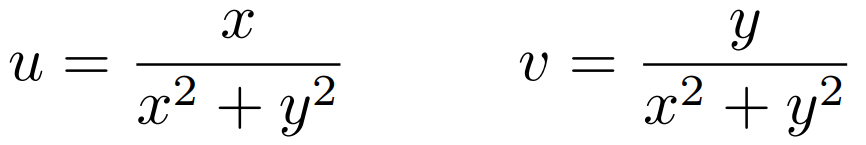
\includegraphics[width=5cm]{other/confCoord.png}};


 \node[inner sep=0pt] (tmp) at (\xRefPosOne-2.7,\yRefPosOne+1)
    {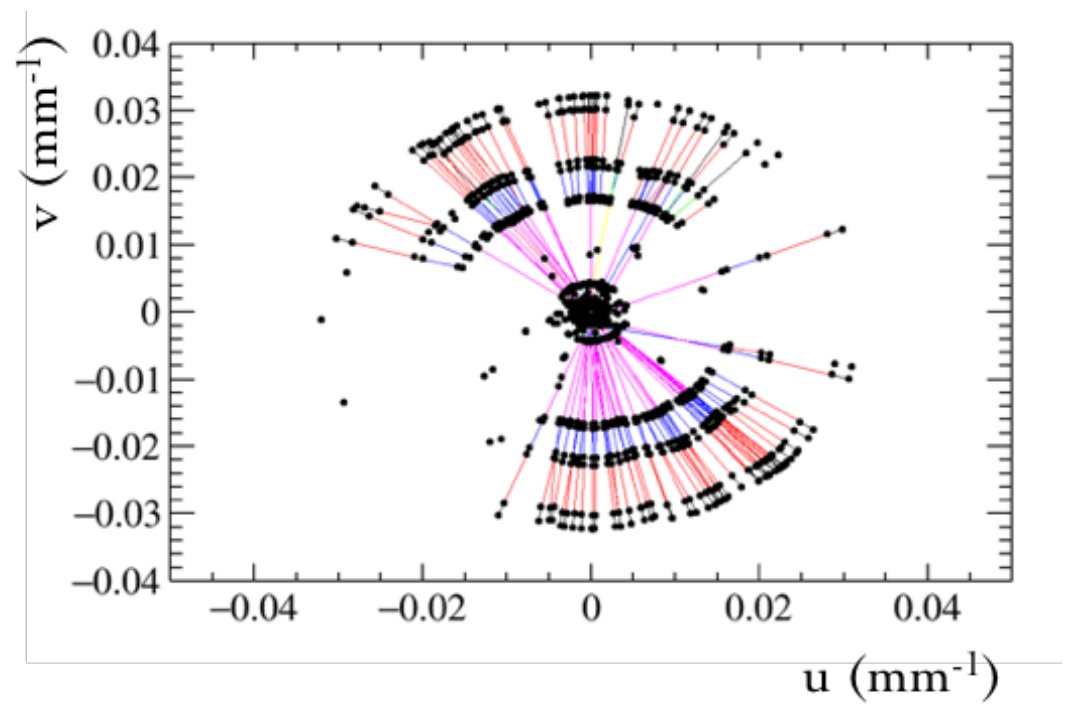
\includegraphics[width=7cm]{other/conformal_tracking.png}};

    
    
\node at (\xRefPosOne,\yRefPosOne-3.5) (box){%
    \begin{minipage}{0.99\textwidth}

  \begin{itemize}
  \item Conformal tracking is used as the main track pattern recognition algorithm at CLIC
 \end{itemize}

    \end{minipage}
};

    
    
\node[inner sep=0pt] (tmp) at (\xRefPosOne,\yRefPosOne-4)
  {\myCenterBox[yellow]{\href{https://agenda.linearcollider.org/event/7645/contributions/40123/attachments/32387/49200/Leogrande_LCWS2017.pdf}
  {{\tiny LCWS presentation about CLIC Conformal Tracking performance }}}  };
  
% \draw[thick,red,rotate=45] (5,5) ellipse (10pt and 20pt);
\draw[thick,red,rotate=20] (4.6,0.15) ellipse (0.52cm and 0.13cm);
\node[right] (textNode) at (6.5,-1) {Hits from the Vertex};
\draw[thick,red,->] (4.8,1.9) to [out=0, in=135]  ([xshift=0.0cm]textNode.west);
  
\draw[thick,red] (2.95,1.3) ellipse (0.5cm and 0.5cm);
\node[right] (textNode) at (0.5,-2) {Hits from the Tracker};
\draw[thick,red,->] (2.45,1.38) to [out=180, in=135]  ([xshift=0.0cm]textNode.west);
  
%% HELPER draw advanced helping grid with axises:
% \draw(-0.5,-4) to[grid with coordinates] (11.5,4);
  
\end{tikzpicture}
  
 
\end{frame}
%*****************************************************************************
%*****************************************************************************
\begin{frame}{\large \large CLD detector layout: x-y view}

\renewcommand{\yRefPosOne}{0}
\renewcommand{\xRefPosOne}{5.5}
\renewcommand{\xRefIncrementOne}{5.5}
\begin{tikzpicture}[overlay]

 \node[inner sep=0pt] (tmp) at (\xRefPosOne-0,\yRefPosOne-0.56)
    {\includegraphics[width=7.8cm]{other/FCC_clic_section.pdf}};


%% HELPER draw advanced helping grid with axises:
% \draw(-0.5,-4) to[grid with coordinates] (11.5,4);
\end{tikzpicture}

 
\end{frame}
%*****************************************************************************
%*****************************************************************************
\begin{frame}{\large \large CLD vs CLICdet overall dimensions}

\renewcommand{\yRefPosOne}{0}
\renewcommand{\xRefPosOne}{5.5}
\renewcommand{\xRefIncrementOne}{5.5}
\begin{tikzpicture}[overlay]

 \node[inner sep=0pt] (tmp) at (\xRefPosOne-0.15,\yRefPosOne-0.9)
    {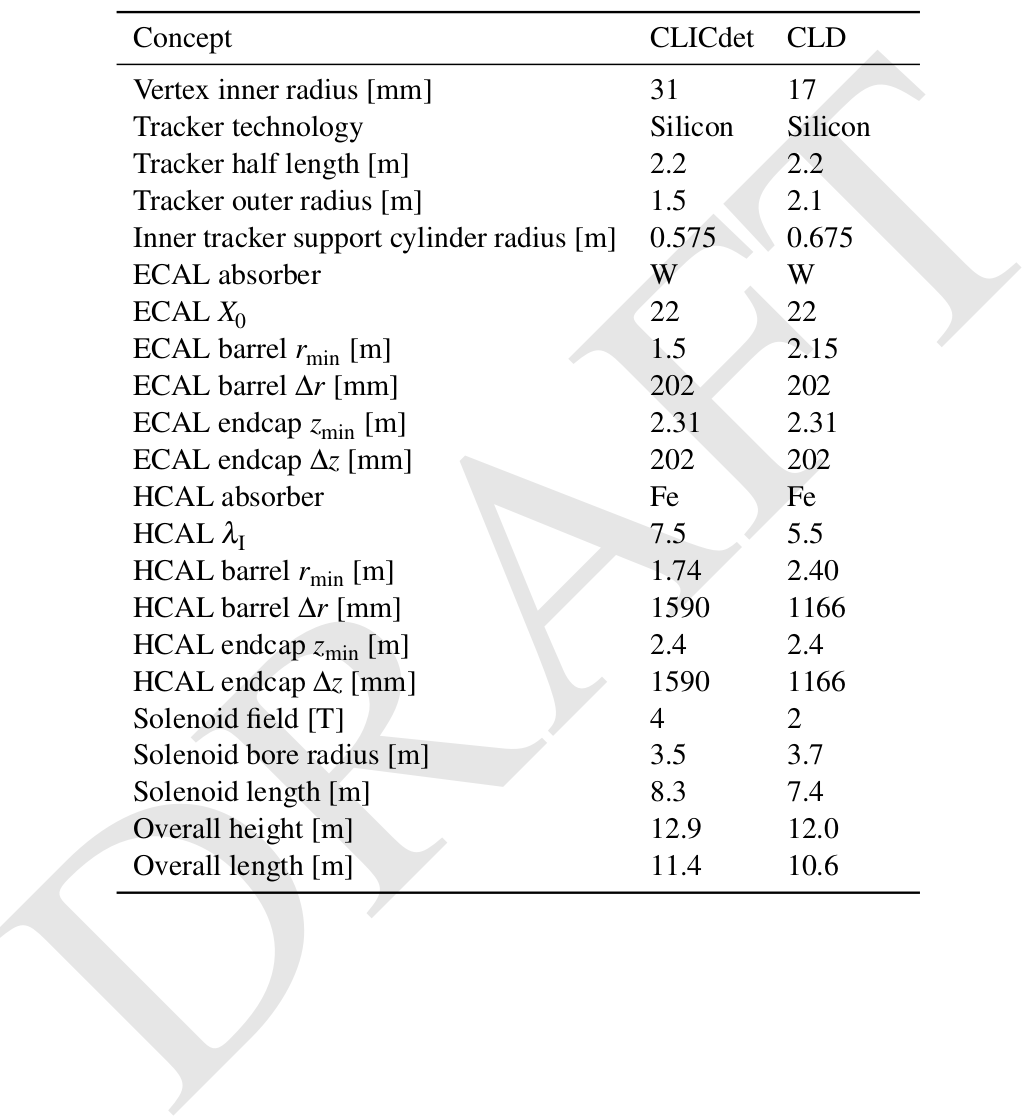
\includegraphics[width=7.8cm]{other/dims.png}};


%% HELPER draw advanced helping grid with axises:
% \draw(-0.5,-4) to[grid with coordinates] (11.5,4);
\end{tikzpicture}

 
\end{frame}
%*****************************************************************************
\backupend

\end{document}

